\documentclass[8pt]{beamer}\usepackage[]{graphicx}\usepackage[]{color}

%\setbeamercovered{transparent}

\usefonttheme{professionalfonts} % using non standard fonts for beamer
\usefonttheme{serif} % default family is serif
\usepackage{fontspec}
\setmainfont{Liberation Serif}

\documentclass{article}
\usepackage{fancyhdr}


\pagestyle{fancy}
\fancyhf{}
\rhead{Ryan Giordano}
\lhead{Research Statement}
\rfoot{Page \thepage}

\usepackage{tabularx}

% \usepackage{fancyhdr}
% \pagestyle{fancy}

% \fancyfoot{}
% \fancyfoot[C]{Rough draft---do not distribute}

\usepackage{etoolbox}


\usepackage{microtype}
\usepackage{graphicx}
\usepackage{subfigure}
\usepackage{booktabs} % for professional tables
\usepackage{xcolor}
\usepackage[hidelinks=True]{hyperref}
\usepackage{xargs}[2008/03/08]

% Documentation
% http://ftp.math.purdue.edu/mirrors/ctan.org/macros/latex/contrib/refstyle/refstyle.pdf
\usepackage{refstyle}
\usepackage{varioref} % Use refstyle instead of varioref directly.

\usepackage{amsmath}
\usepackage{amssymb}
\usepackage{amsfonts}
\usepackage{amsthm}
\usepackage{mathrsfs} % For mathscr
\usepackage{mathtools}

\usepackage[authoryear]{natbib}
\bibliographystyle{apalike}

\usepackage{geometry}
\geometry{margin=1.5in}

% % This file contains the boilerplate that knitr would put at the top of
% a knitr document if you ran knitr with \begin{document} ... \end{document}.
% By including it once in the main document, you can knit and \input{}
% Rnw files that contain only individual sections.

\usepackage[]{graphicx}
\usepackage[]{color}
%% maxwidth is the original width if it is less than linewidth
%% otherwise use linewidth (to make sure the graphics do not exceed the margin)
\makeatletter
\def\maxwidth{ %
  \ifdim\Gin@nat@width>\linewidth
    \linewidth
  \else
    \Gin@nat@width
  \fi
}
\makeatother

\definecolor{fgcolor}{rgb}{0.345, 0.345, 0.345}
\newcommand{\hlnum}[1]{\textcolor[rgb]{0.686,0.059,0.569}{#1}}%
\newcommand{\hlstr}[1]{\textcolor[rgb]{0.192,0.494,0.8}{#1}}%
\newcommand{\hlcom}[1]{\textcolor[rgb]{0.678,0.584,0.686}{\textit{#1}}}%
\newcommand{\hlopt}[1]{\textcolor[rgb]{0,0,0}{#1}}%
\newcommand{\hlstd}[1]{\textcolor[rgb]{0.345,0.345,0.345}{#1}}%
\newcommand{\hlkwa}[1]{\textcolor[rgb]{0.161,0.373,0.58}{\textbf{#1}}}%
\newcommand{\hlkwb}[1]{\textcolor[rgb]{0.69,0.353,0.396}{#1}}%
\newcommand{\hlkwc}[1]{\textcolor[rgb]{0.333,0.667,0.333}{#1}}%
\newcommand{\hlkwd}[1]{\textcolor[rgb]{0.737,0.353,0.396}{\textbf{#1}}}%
\let\hlipl\hlkwb

\usepackage{framed}
\makeatletter
\newenvironment{kframe}{%
 \def\at@end@of@kframe{}%
 \ifinner\ifhmode%
  \def\at@end@of@kframe{\end{minipage}}%
  \begin{minipage}{\columnwidth}%
 \fi\fi%
 \def\FrameCommand##1{\hskip\@totalleftmargin \hskip-\fboxsep
 \colorbox{shadecolor}{##1}\hskip-\fboxsep
     % There is no \\@totalrightmargin, so:
     \hskip-\linewidth \hskip-\@totalleftmargin \hskip\columnwidth}%
 \MakeFramed {\advance\hsize-\width
   \@totalleftmargin\z@ \linewidth\hsize
   \@setminipage}}%
 {\par\unskip\endMakeFramed%
 \at@end@of@kframe}
\makeatother

\definecolor{shadecolor}{rgb}{.97, .97, .97}
\definecolor{messagecolor}{rgb}{0, 0, 0}
\definecolor{warningcolor}{rgb}{1, 0, 1}
\definecolor{errorcolor}{rgb}{1, 0, 0}
\newenvironment{knitrout}{}{} % an empty environment to be redefined in TeX

\usepackage{alltt}



\def\argmax#1{\mathrm{argmax}_{#1}\,}
\def\argmin#1{\mathrm{argmin}_{#1}\,}
\def\cov#1#2{\mathrm{Cov}_{#1}\left( #2\right)\,}
\def\expect#1#2{\mathbb{E}_{#1}\left[ #2\right]\,}
\def\var#1#2{\mathrm{Var}_{#1}\left( #2\right)\,}
\def\cumulant#1#2{\mathcal{K}_{#1}\left( #2\right)\,}
\def\expecthat#1#2{\hat{\mathbb{E}}_{#1}\left[ #2\right]\,}
\newcommand{\fracat}[3]{\left. \frac{#1}{#2} \right|_{#3}}
\newcommand{\norm}[1]{\left\Vert#1\right\Vert}
\newcommand{\abs}[1]{\left|#1\right|}
\def\diag#1{\textrm{Diag}\left( #1\right)}
\def\ord#1{\mathcal{O}\left( #1\right)}
\def\ordp#1{\mathcal{O}_p\left( #1\right)}
\def\gauss#1{\mathcal{N}\left( #1\right)}
\def\trans{\intercal} % transpose
\def\id{I} % Identity matrix
\def\iid{\overset{iid}{\sim}}
\def\rdom#1{\mathbb{R}^{#1}}
\def\ind#1{\mathbb{I}\left(#1\right)}
\def\varemp#1{\hat{\mathrm{Var}}\left(#1\right)}


% Sets of data in the survey and target

\def\tarcol#1{\textcolor{red}{#1}}
\def\surcol#1{\textcolor{blue}{#1}}


\def\sur{\mathcal{S}}
\def\tar{\mathcal{T}}
\def\nsur{{\surcol{N_S}}}
\def\ntar{{\tarcol{N_T}}}

\def\Nsur{{\surcol{N_S}}}
\def\Ntar{{\tarcol{N_T}}}


\def\postsur{\surcol{\p(\theta \vert \textrm{Survey data})}}
\def\post{\postsur}

\def\f{f}
\def\sumn{\sum_{n=1}^N}
\def\meann{\frac{1}{N} \sum_{n=1}^N}
\def\sumsur{\sum_{i=1}^\Nsur}
\def\sumtar{\sum_{j=1}^\Ntar}
\def\meansur{\frac{1}{\Nsur} \sumsur}
\def\meantar{\frac{1}{\Ntar} \sumtar}


% Distributions of x or (x, y) in the survey and target
% p is common to both (for p(y | x))
\def\psur{\surcol{{\mathcal{P}_{S}}}}
\def\ptar{\tarcol{\mathcal{P}_{T}}}
%\def\ptarhat{{\hat{\mathcal{P}}_{T}}}
\def\p{\mathcal{P}}
%\def\post{\p(\beta \vert \sur )}
\newcommand{\postd}[1][\delta]{\p(\beta \vert \sur, #1)}



% Different MrP estimates
\def\mrp{\mathrm{MrP}}
\def\ols{\mathrm{OLS}}
\def\cal{\mathrm{WGT}}
\def\glm{\mathrm{GLM}}
\def\hwt{\mathrm{HT}} % Horwitz--Thompson

% Population estimator
\newcommand{\muhat}[1][]{\hat{\mu}^{#1}}
\newcommand{\w}[1][]{w^{#1}}

\newcommand{\muhatmrp}[1][\Ysur]{\tarcol{\muhat[\mrp]}(\surcol{#1})}
\newcommand{\muhatcw}[1][\Ysur]{\tarcol{\muhat[\cal]}(\surcol{#1})}


% Link function, usually expit.
\def\m{m}
\def\mhat{\hat{\m}}
\def\minv{\m^{-1}}
\def\betahat{\hat{\beta}} % Regression coefficient
\def\betastar{\overset{*}{\beta}} % Regression coefficient
\def\betadom{\rdom{D_\beta}}
% \def\thetahat{\hat{\theta}} % All parameters
% \def\thetastar{\overset{*}{\theta}} % All parameters

% BCLT quantities
\def\g{g} % Quantity of interest
\def\info{\mathcal{I}}
\def\infohat{\hat{\info}}
\def\resid{\mathcal{E}}
\def\V{V} % Limiting variance
\def\Vhat{\hat{V}} % Limiting variance estimate

\def\tautil{\tilde{\tau}} % Intermediate value for covariate balance
\def\A{A} % Log partition function
\def\Ap{A^{+}} % Log partition function
\def\Agrad#1{A_{(#1)}} % Log partition function derivative
\def\betaball{\mathcal{B}_{\delta}} % Neighborhood of thetastar
\def\deltamax{\delta_{+}} % Maximum value of \delta
\def\deltadom{[0, \deltamax]} % Maximum value of \delta

% % Estimating equation
% \def\G{G}
% \def\H{H}
% \def\Hhat{\hat{H}}
% \def\t{t} % Implicit function theorem perturbation


% Different "weights"


\def\thetahat{\hat{\theta}}

% The regressors actually used in MrP (as opposed to x)
% which is all observed data.
\def\Ztar{Z_{\tar}}
\def\Zsur{Z_{\sur}}
\def\z{z}

% THe full observed regressors, possibly distinct from what 
% is actually in the regression
\def\x{\mathbf{x}}
\def\X{X}
\def\Xtar{X_{\tar}}
\def\Xsur{X_{\sur}}


% The response weighting error
\def\r{r}  % New (missing) regressor
\def\rdim{D_r}  % New (missing) regressor
\def\Rsur{R_{\sur}}  % New (missing) sample regressor
\def\Rtar{R_{\tar}}  % New (missing) target regressor

% % dyhat / dy
% \def\W{W}
\def\w{w}
\def\wmrp{w^{\mrp}}
\def\wv{\mathbf{w}}
% \def\Wols{W_{OLS}}
% \def\Wglm{W_{GLM}}
% \def\Wbhm{W_{BHM}}


% The response vector and values
\def\y{y}
\def\yhat{\hat{y}}
\def\ytil{\tilde{y}}
\def\Ytil{\tilde{Y}}
\def\Yhat{\hat{Y}}
\def\Ysur{\surcol{Y_{\sur}}}
\def\Ytil{\surcol{\tilde{Y}_{\sur}}}



\def\splitpage#1#2{
\begin{minipage}[t]{0.45\textwidth}
    #1
\end{minipage}
\hfill\vrule\hfill
\begin{minipage}[t]{0.45\textwidth}
    #2
\end{minipage}
}

\def\splitpagenoline#1#2{
\begin{minipage}[t]{0.45\textwidth}
    #1
\end{minipage}
\hfill
\begin{minipage}[t]{0.45\textwidth}
    #2
\end{minipage}
}
%%%%%%%%%%%%%%%%%%%%%%%%%%%%%%%%%%%%%%
%%%%%%%%%%%%%%%%%%%%%%%%%%%%%%%%%%%%%%
% Do not edit the TeX file your work
% will be overwritten.  Edit the RnW
% file instead.
%%%%%%%%%%%%%%%%%%%%%%%%%%%%%%%%%%%%%%
%%%%%%%%%%%%%%%%%%%%%%%%%%%%%%%%%%%%%%





%%%%%%%%%%%%%%%%%%%%%%
%%%%%%%%%%%%%%%%%%%%%%
%%%%%%%%%%%%%%%%%%%%%%
% Plots

\newcommand{\BaseHistogram}{
\begin{knitrout}
\definecolor{shadecolor}{rgb}{0.969, 0.969, 0.969}\color{fgcolor}

{\centering 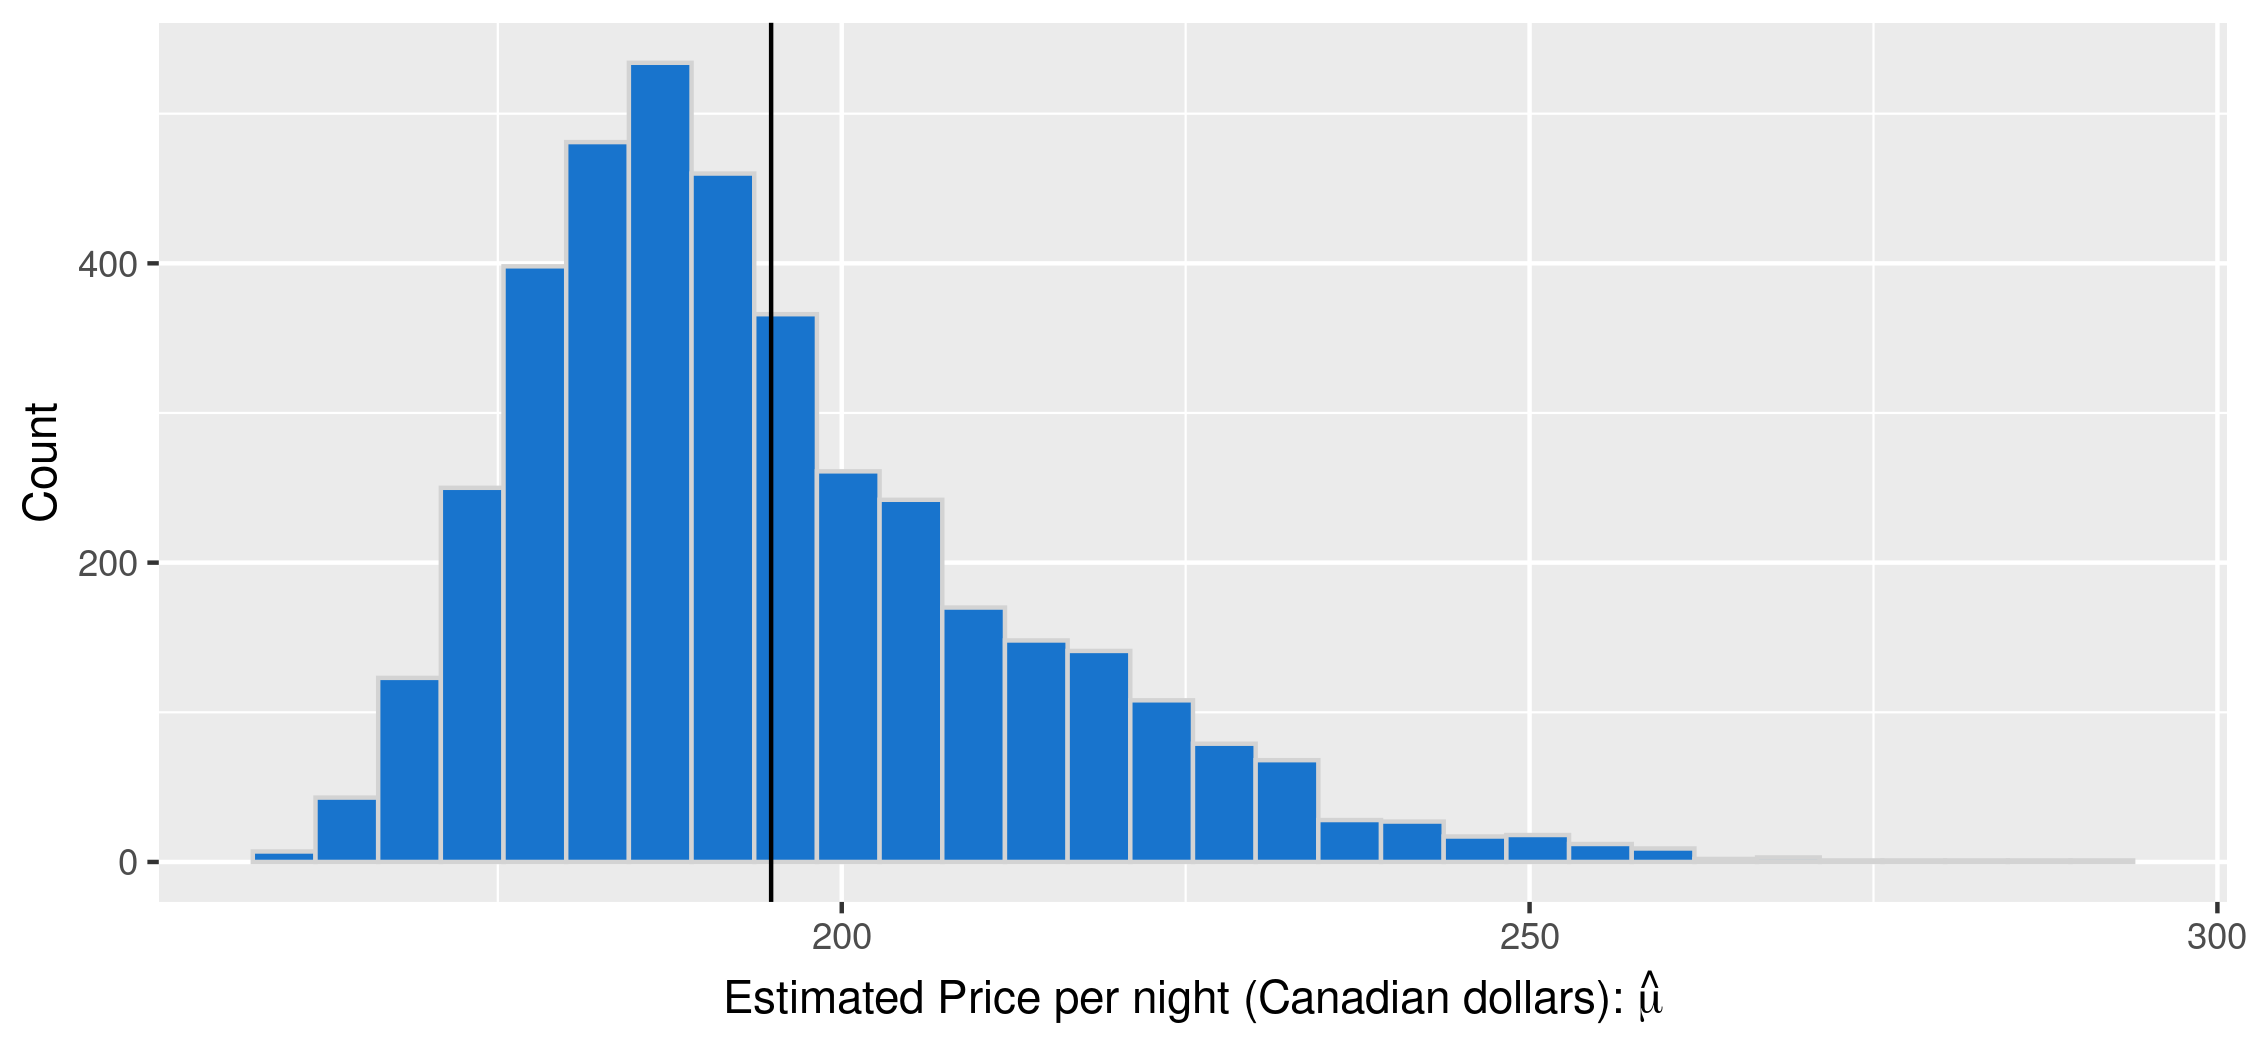
\includegraphics[width=0.98\linewidth,height=0.461\linewidth]{figure/base-hist-1} 

}



\end{knitrout}
}


\newcommand{\BaseHistogramWithArrow}{
\begin{knitrout}
\definecolor{shadecolor}{rgb}{0.969, 0.969, 0.969}\color{fgcolor}

{\centering 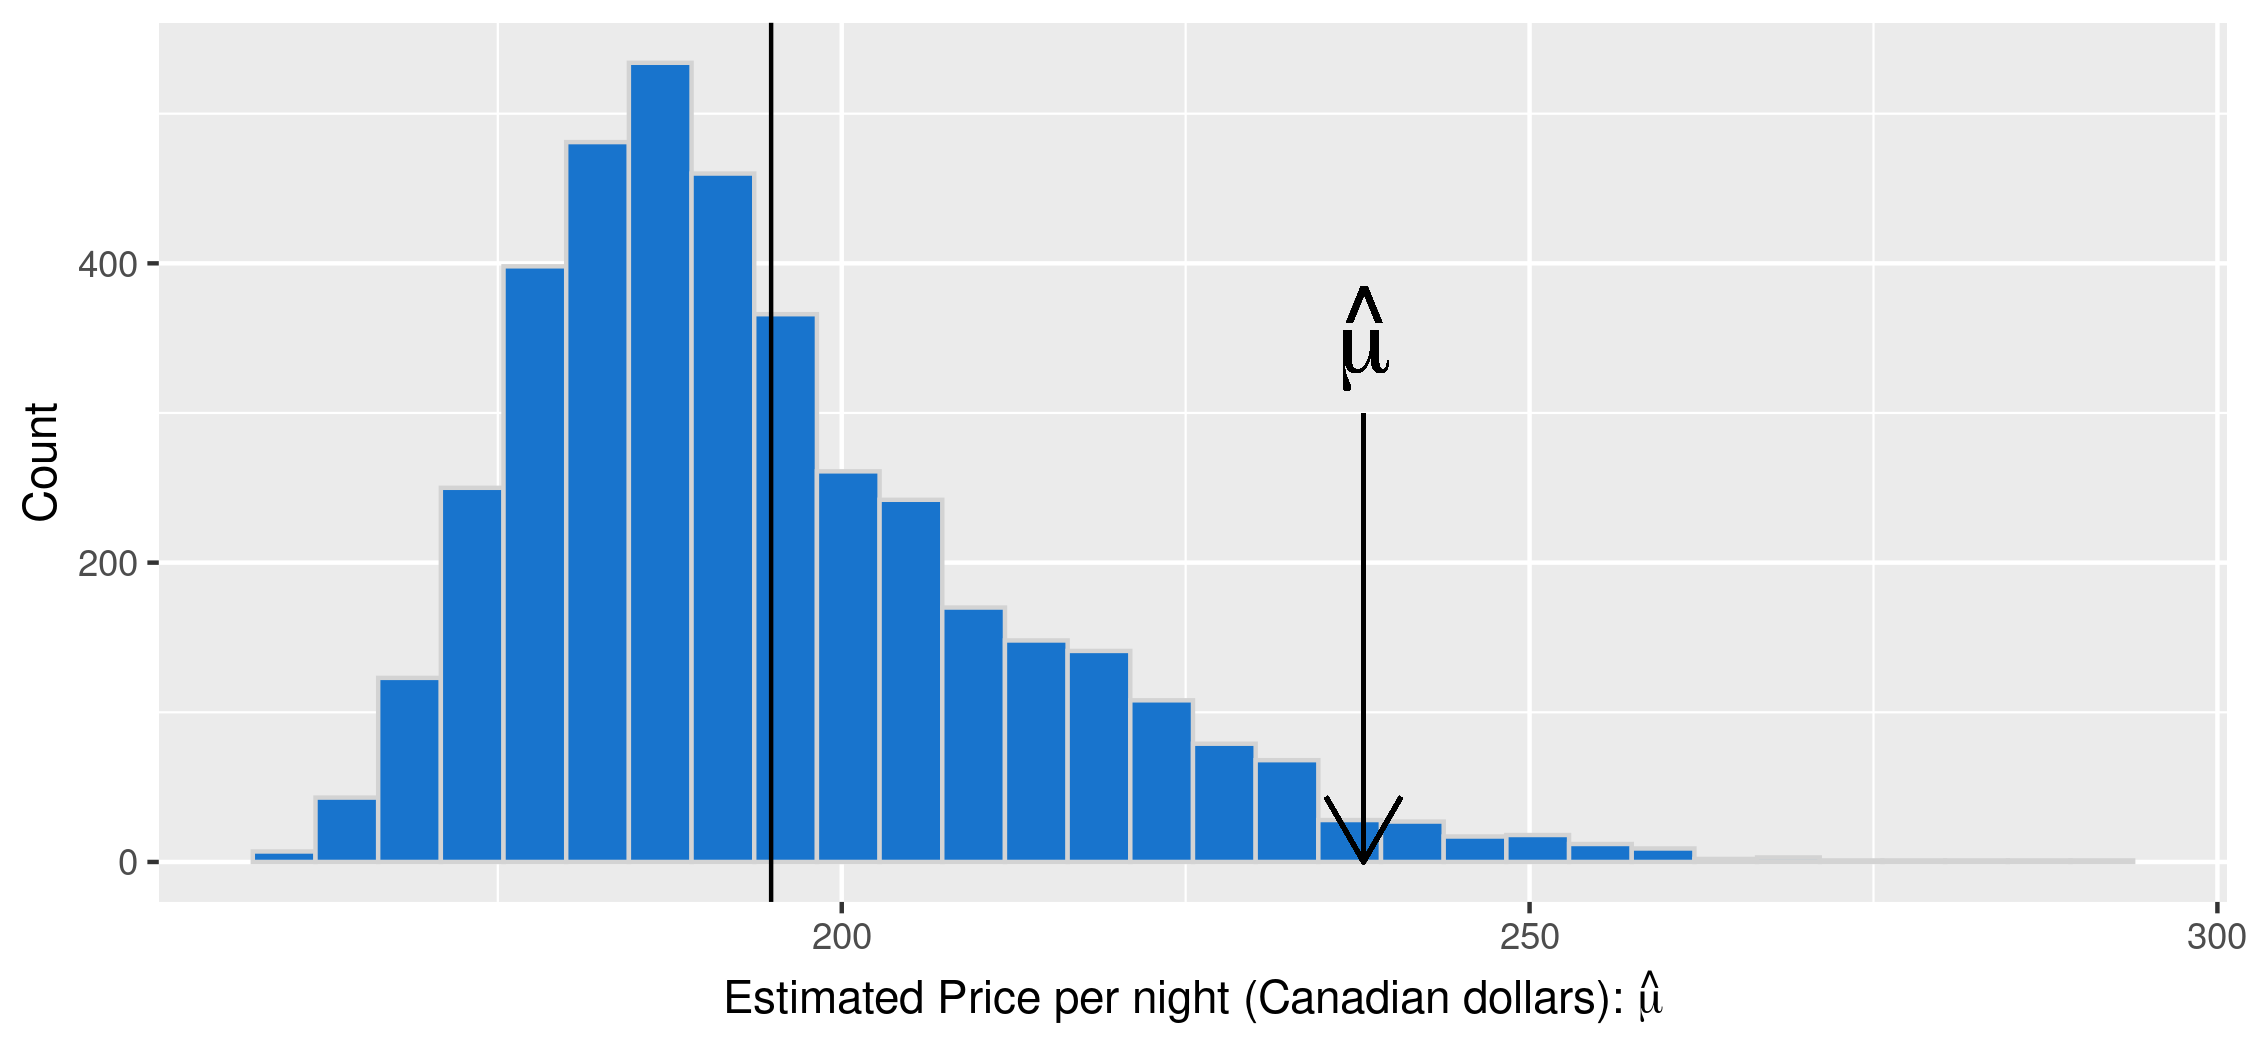
\includegraphics[width=0.98\linewidth,height=0.461\linewidth]{figure/base-hist-arrow-1} 

}



\end{knitrout}
}



\newcommand{\BaseHistogramFaded}{
\begin{knitrout}
\definecolor{shadecolor}{rgb}{0.969, 0.969, 0.969}\color{fgcolor}

{\centering 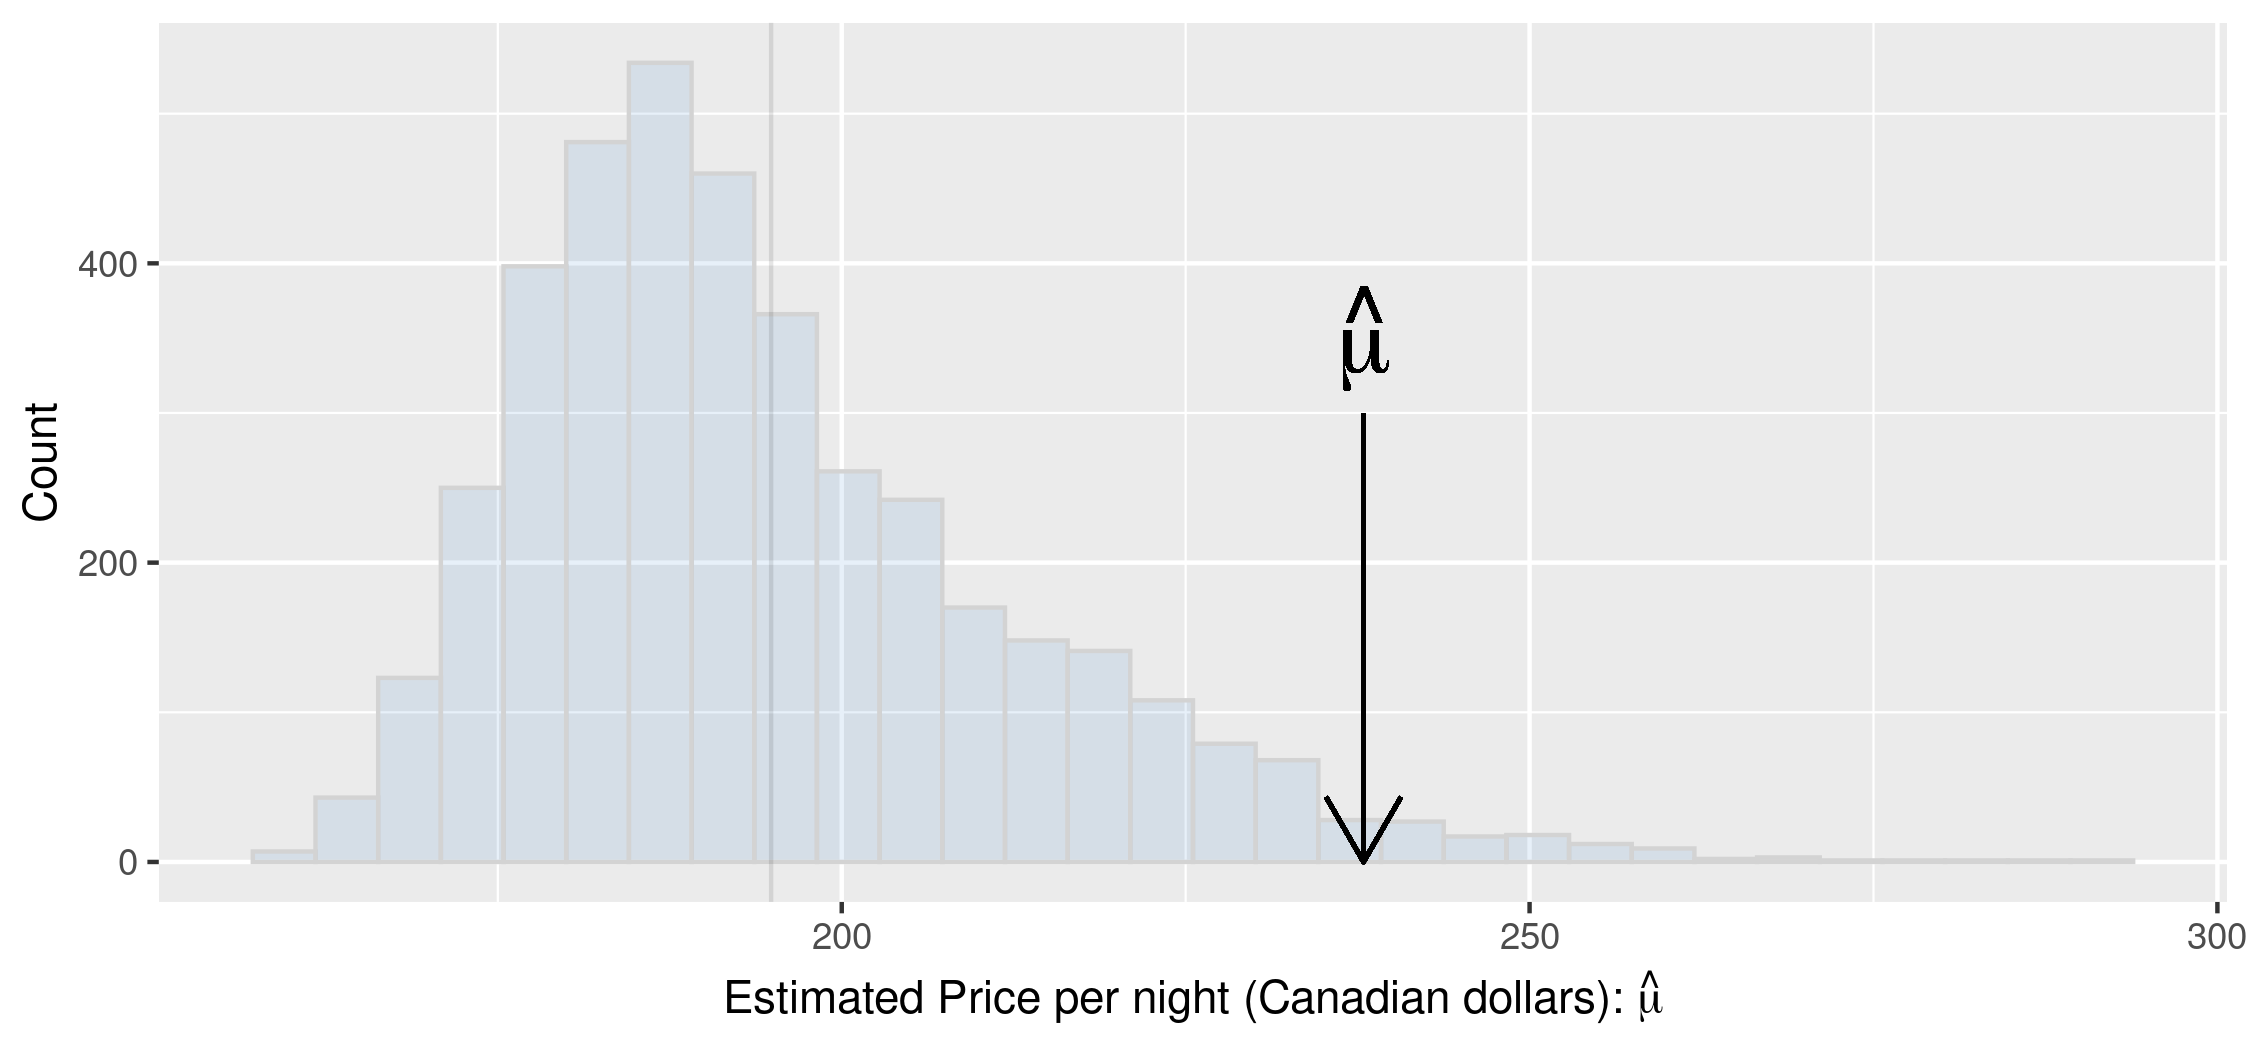
\includegraphics[width=0.98\linewidth,height=0.461\linewidth]{figure/base-hist-faded-1} 

}



\end{knitrout}
}


\newcommand{\SingleCI}{
\begin{knitrout}
\definecolor{shadecolor}{rgb}{0.969, 0.969, 0.969}\color{fgcolor}

{\centering 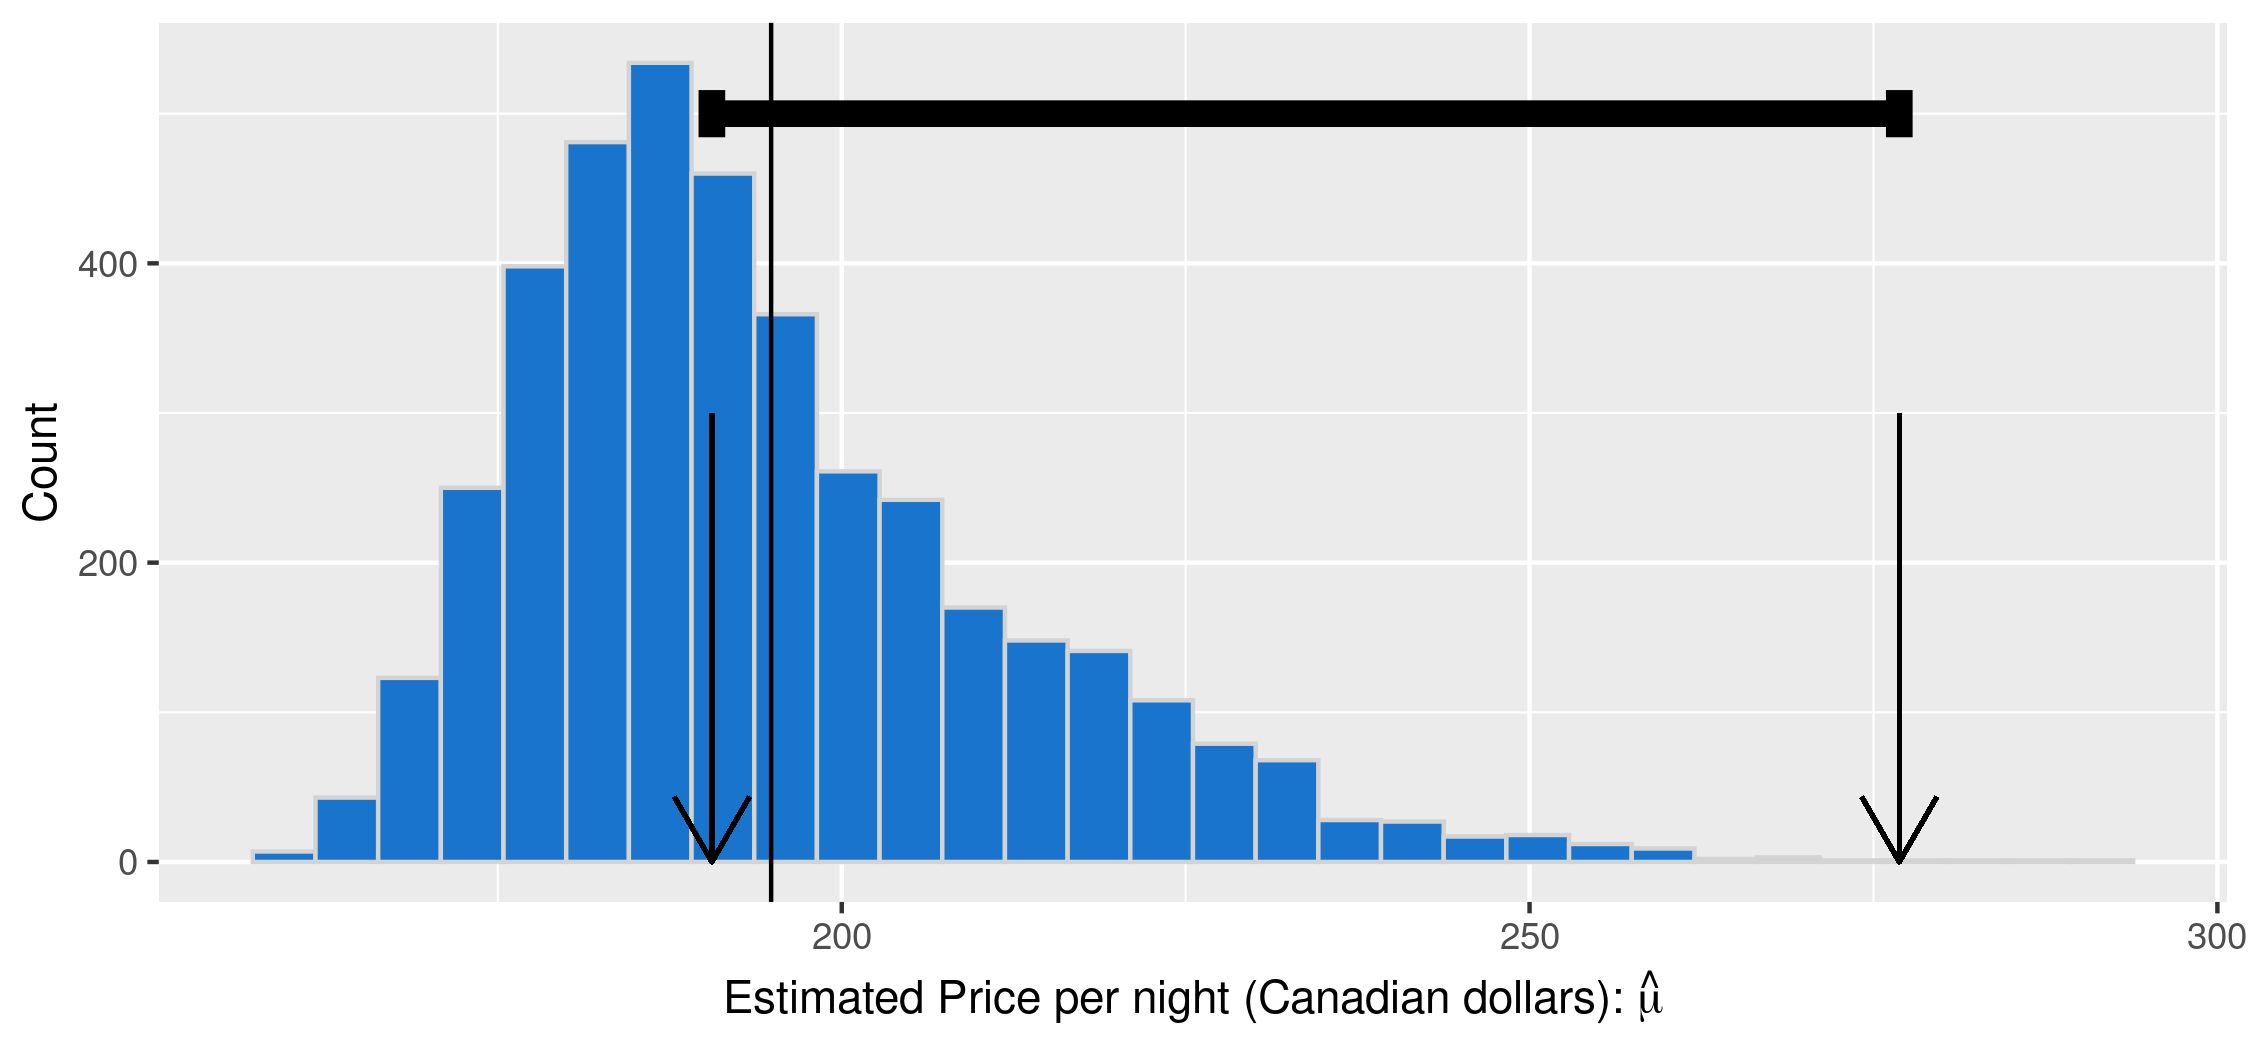
\includegraphics[width=0.98\linewidth,height=0.461\linewidth]{figure/base-hist-ci-1} 

}



\end{knitrout}
}




\newcommand{\SingleCIB}{
\begin{knitrout}
\definecolor{shadecolor}{rgb}{0.969, 0.969, 0.969}\color{fgcolor}

{\centering 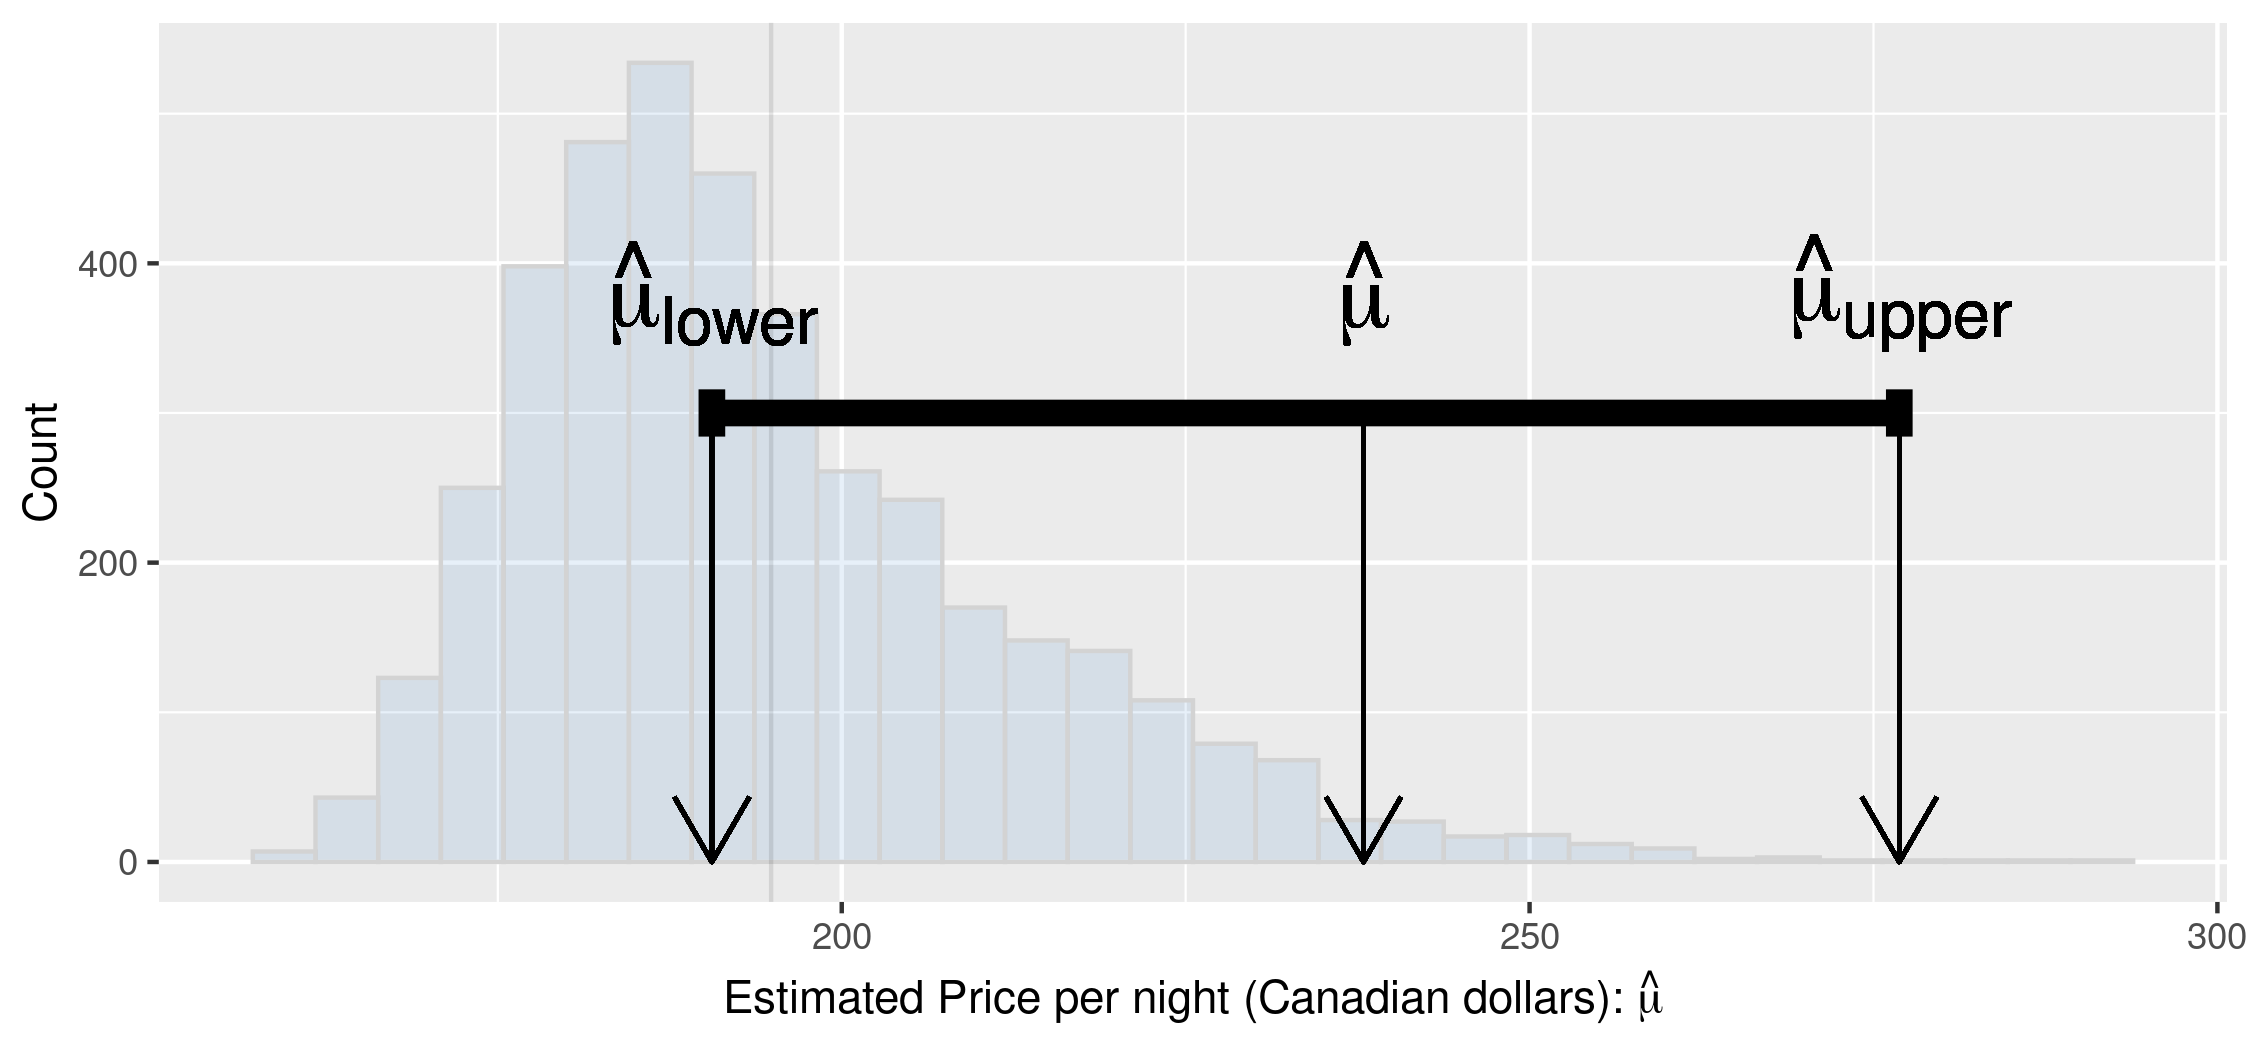
\includegraphics[width=0.98\linewidth,height=0.461\linewidth]{figure/base-hist-cib-1} 

}



\end{knitrout}
}



\newcommand{\MultipleCIs}{



\begin{knitrout}
\definecolor{shadecolor}{rgb}{0.969, 0.969, 0.969}\color{fgcolor}

{\centering 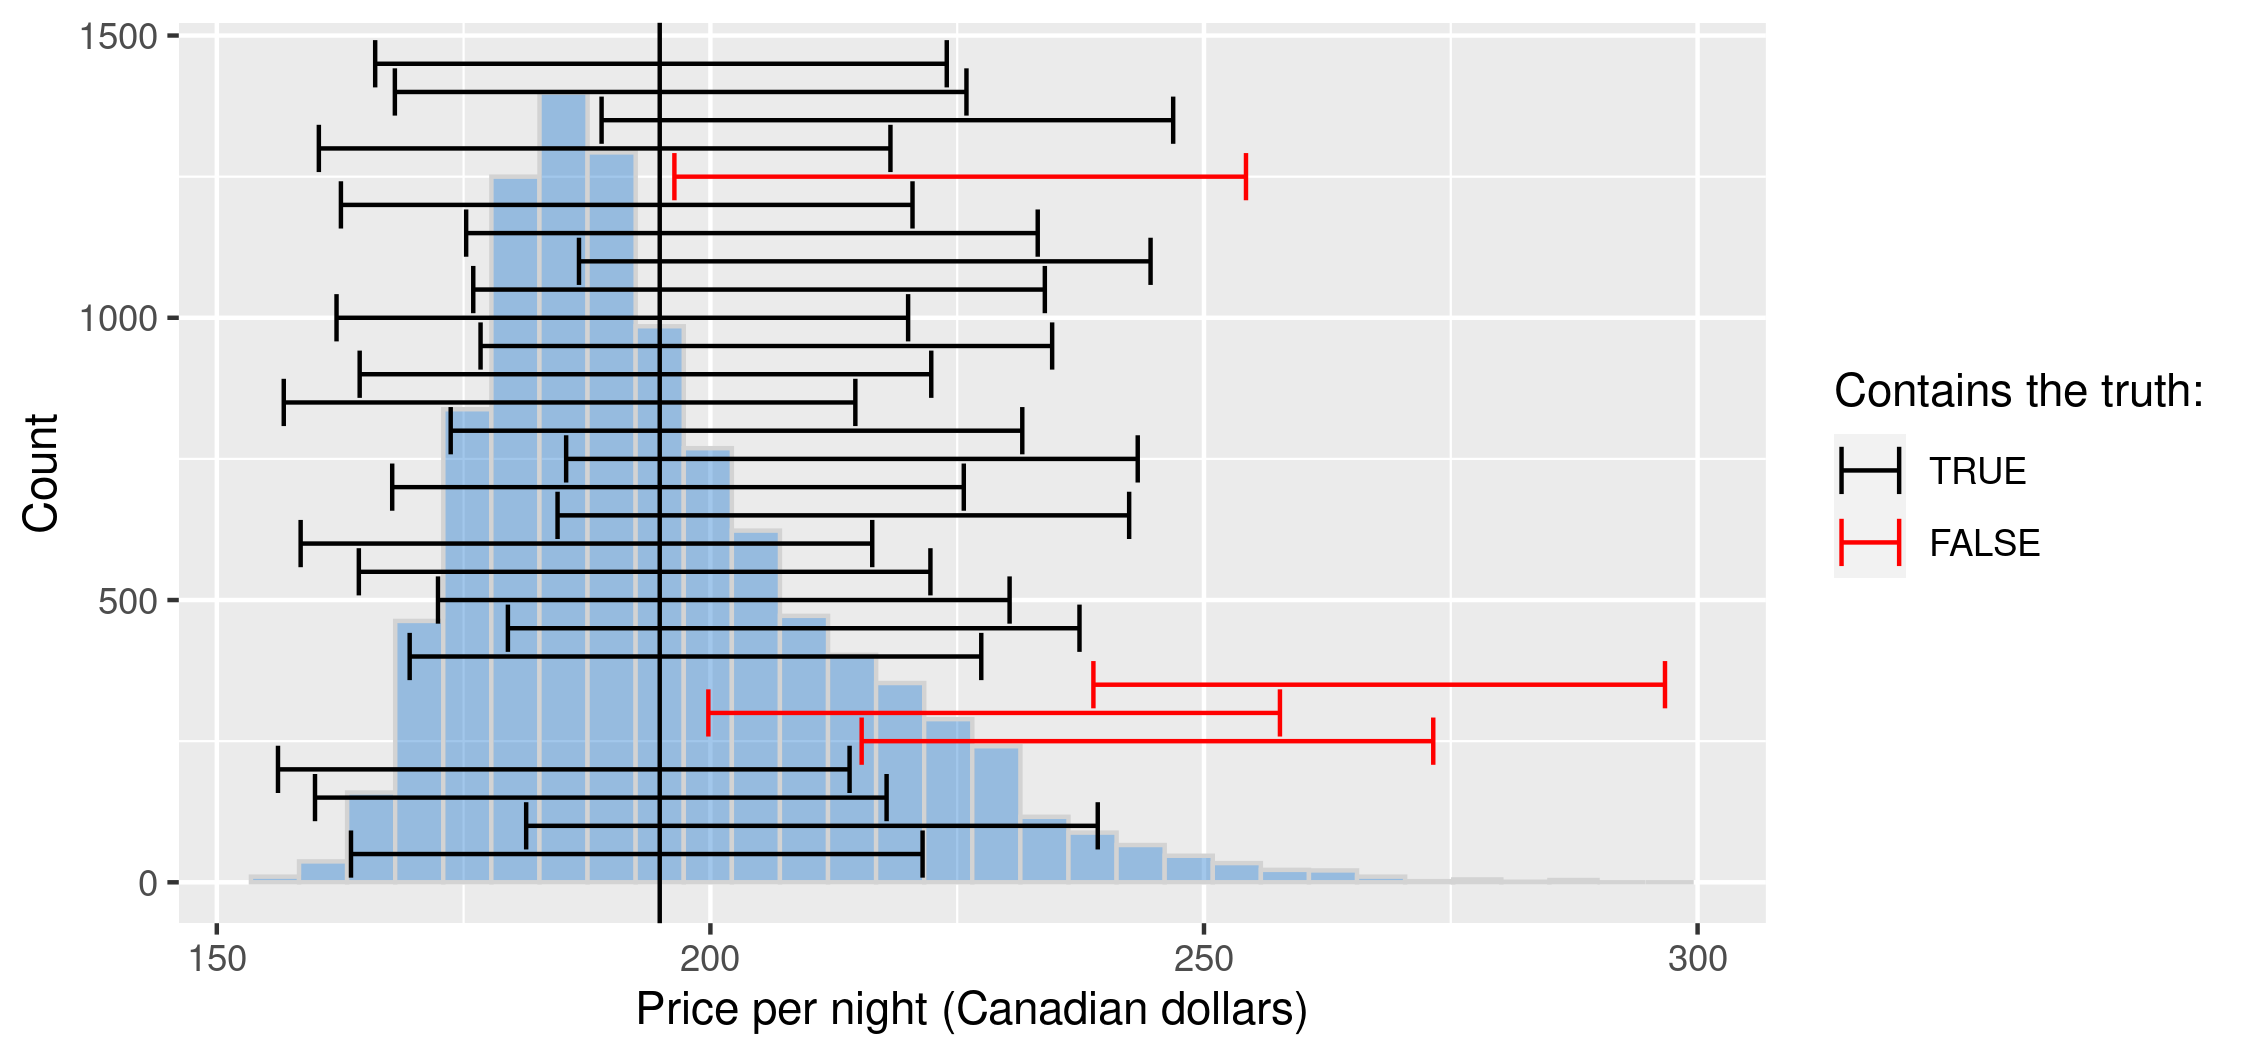
\includegraphics[width=0.98\linewidth,height=0.461\linewidth]{figure/base-hist-cis-1} 

}



\end{knitrout}
}


\DefineMacros{}

\title{Weighting-Like Diagnostics for Nonlinear \\Bayesian Hierarchical Models}
\author{Ryan Giordano, Alice Cima, Erin Hartman, Jared Murray, Avi Feller}

\date{\textbf{October 2025 Stanford Berkeley Joint Colloquium}}

% \titlegraphic{
%     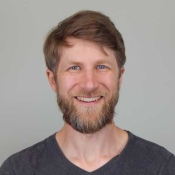
\includegraphics[width=0.2\textwidth]{static_figures/ryan_giordano.jpeg}
% }

\setbeamertemplate{Collaborators}[none]
\IfFileExists{upquote.sty}{\usepackage{upquote}}{}


 \institute{
    \centering
    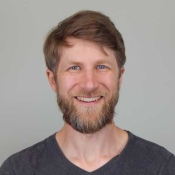
\includegraphics[height=0.15\textwidth]{static_figures/ryan_giordano.jpeg}
    
\includegraphics[height=0.15\textwidth]{static_figures/alice.jpg}
    
\includegraphics[height=0.15\textwidth]{static_figures/erin_hartman.jpg}
    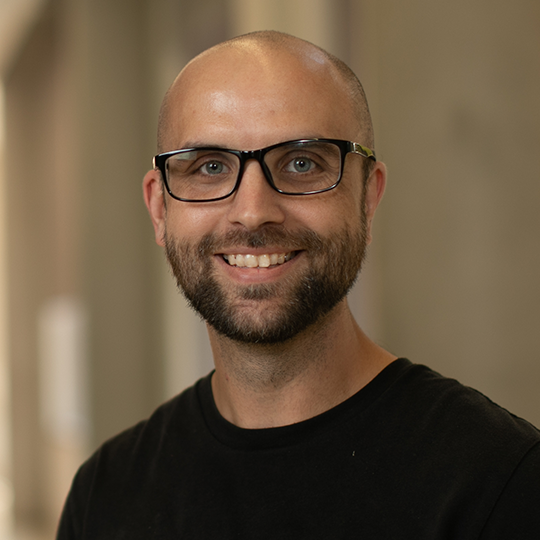
\includegraphics[height=0.15\textwidth]{static_figures/jared_murray.png}
    
\includegraphics[height=0.15\textwidth]{static_figures/avi_feller.jpg}
 }

\begin{document}

\maketitle


\def\sectionslide#1{
\begin{frame}
   \centering
   \huge{\textbf{#1}}
\end{frame}
}



\begin{frame}{Mister freakin P}


\end{frame}






\begin{frame}{The basic problem}

%\adjincludegraphics[width=0.9\textwidth,trim={0 {.5\height} 0 0 }, clip]{static_figures/survey_and_voting.jpg}

We have a survey population, for whom we observe:
%
\begin{itemize}
 \item Covariates $\x$ (e.g.~race, gender, zip code, age, education level)
 \item Responses $\y$ (e.g.~A binary response to ``do you support candidate Z'')
\end{itemize}
%

We want the average response in a target population,
in which we observe only covariates.


\splitpage{
    \centering
    \only<1>{
    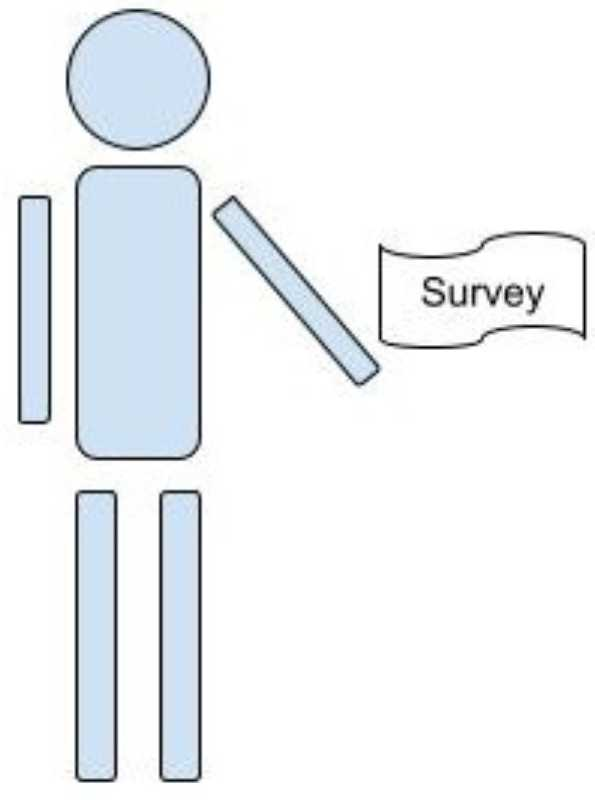
\includegraphics[width=0.5\textwidth]{static_figures/survey_man.jpg}
    }
    \only<2->{
    %
\includegraphics[width=0.5\textwidth]{static_figures/survey_crazy_man.jpg}
    
\includegraphics[width=0.5\textwidth]{static_figures/guinea_pig.png}
    }
}{
    \centering
    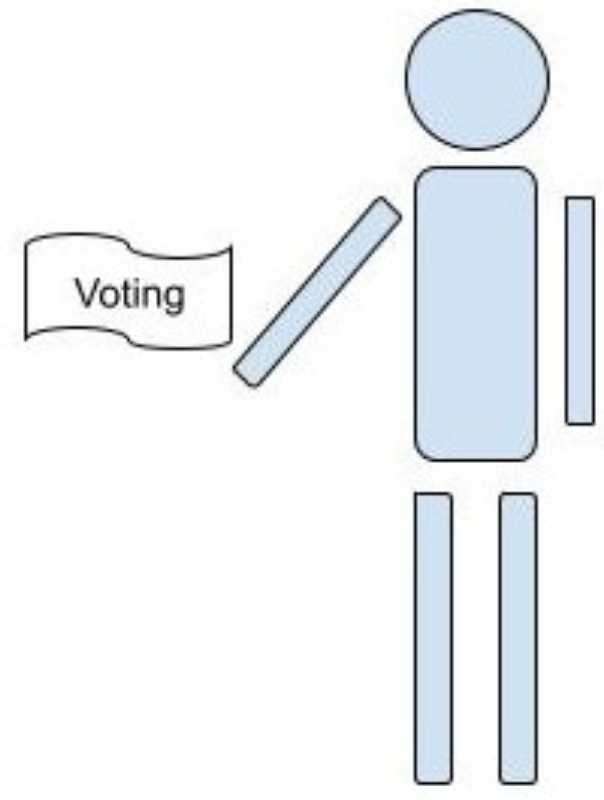
\includegraphics[width=0.5\textwidth]{static_figures/voting_man.jpg}
}

\splitpage{
    \centering
    Observe \surcol{$(\x_i, y_i)$ for $i = 1, \ldots, \nsur$}\\
}{
    \centering
    Observe \tarcol{$\x_j$ for $j = 1, \ldots, \ntar$}\\
}

\onslide<2->{
\textbf{The problem is that the populations may be very different, maybe leading to bias.}
\footnote{Photo copyright: Mark Taylor / \texttt{naturepl.com}}
}

\onslide<3->{
    How can we use the covariates
    to say something about the target responses?
}
%
\end{frame}

%%%%%%%%%%%%%%%%%%%%%%%%%%%%%%%%%%%%%%%%%%%%%%%%%%%%%%%
%%%%%%%%%%%%%%%%%%%%%%%%%%%%%%%%%%%%%%%%%%%%%%%%%%%%%%%
%%%%%%%%%%%%%%%%%%%%%%%%%%%%%%%%%%%%%%%%%%%%%%%%%%%%%%%

\begin{frame}[t]{Two approaches}

We want $\tarcol{\mu := \meantar \y_j}$,
but don't observe target $\tarcol{\y_j}$.  Let $\surcol{\Ysur = \{\y_1, \ldots, \y_{\Nsur}\}}$.

\begin{itemize}
    \item Assume $p(y | \x)$ is the same in both populations,
    \item But the distribution of $\x$ may be different in the survey and target.
\end{itemize}
%
\pause

\splitpagenoline{
    \centering
    \textbf{Calibration weighting}
}{
    \centering
    %\textbf{Multilevel regression and poststratification (MrP)}
    \textbf{Bayesian hierarchical modeling (MrP)}
}
%
%\\\hrulefill\\
\\[1em]
%
\splitpagenoline{
    \centering
    $\blacktriangleright$
    Choose ``calibration weights'' \surcol{$w_i$}\\
    using only the regressors $\x$\\
    (e.g.~raking weights)
}{
    \centering
    $\blacktriangleright$
    Choose $\expect{}{\y \vert \x, \theta} = m(\theta^\trans \x)$,\\
    choose prior $\p(\theta | \Sigma) \p(\Sigma)$\\
    (e.g.~Hierarchical logistic regression)
} \pause
%
\\[1em]
\splitpagenoline{
    \centering
    $\blacktriangleright$ Take
    $\muhatcw = \surcol{\meansur w_i y_i}$
}{
    \centering
    $\blacktriangleright$ Take
    $\tarcol{\yhat_j} =
        \expect{\postsur}{\y | \tarcol{\x_j}}$ and\\
    $\muhatmrp = \tarcol{\meantar \yhat_j}$
}\pause
%
\\[1em]
\splitpagenoline{
    \centering
    $\blacktriangleright$ Dependence %of \surcol{$\muhat_{\cal}$}
    on \surcol{$\y_i$} is clear\\
    % (\surcol{$\w_i$} typically chosen using only $\x$)
}{
    \centering
    $\blacktriangleright$ Dependence %of \surcol{$\muhat_\mrp$}
    on \surcol{$\y_i$} very complicated\\
    (Typically via MCMC draws from $\postsur$)
}\pause
%
\\[1em]
\splitpagenoline{
    \centering
    $\blacktriangleright$ Weights give interpretable diagnostics:
    %
    \begin{itemize}
        \item Frequentist variability
        \item Regressor balance
        \item Partial pooling
        %\item Extrapolation
    \end{itemize}
    %
}{
    \centering
    $\blacktriangleright$ \textbf{Black box}\\
    \pause
    \vspace{1em}
    $\leftarrow$ Today, we'll open the box and provide
        MrP analogues of all these diagnostics
}


\end{frame}


%%%%%%%%%%%%%%%%%%%%%%%%%%%%%%%%%%%%%%%%%%%%%%%%%%%%%%%
%%%%%%%%%%%%%%%%%%%%%%%%%%%%%%%%%%%%%%%%%%%%%%%%%%%%%%%
%%%%%%%%%%%%%%%%%%%%%%%%%%%%%%%%%%%%%%%%%%%%%%%%%%%%%%%

\begin{frame}{Prior work: Equivalent weights for linear models}

\textcite{gelman:2007:struggles} observes that MrP is a weighting estimator when
$\yhat$ is computed with OLS:
$$
\begin{aligned}
% \yhat_j ={}& \x_j^\trans \thetahat  =
%     \x_j^\trans \left(\sumsur \x_i \x_i^\trans \right)^{-1} \sumsur \x_i \y_i \Rightarrow \\
\muhatmrp ={}& \tarcol{\meantar \yhat_j} =
\tarcol{\meantar }
\underbrace{\tarcol{\x_j^\trans} \surcol{\betahat}}_{\textrm{Linear in }\surcol{\Ysur}}
% =
% \surcol{\sumsur}
% \underbrace{
% \left(\tarcol{\meantar \x_j^\trans}
%     \surcol{
%         \left(\sum_{i'=1}^{\Nsur} \x_{i'} \x_{i'}^\trans \right)^{-1} \x_i
%     }
% \right)
% }_{\surcol{\w^\mrp_i}}  \surcol{\y_i} \\
\end{aligned}
$$

Most existing literature on comparing weighting and MrP focus on such linear models.
\footnote{
    For example,
    \textcite{gelman:2007:struggles,benmichael:2021:multilevel,chattopadhyay:2023:implied}.}

\onslide<2->{
But what if you use a non--linear link function?  Or a hierarchical model?\\
\vspace{2em}
\hrulefill
\begin{displayquote}
``It would also be desirable to use nonlinear methods  ...
but then it would seem difficult to construct
even approximately equivalent weights.  Weighting and fully nonlinear models
would seem to be completely incompatible methods.''
--- \parencite{gelman:2007:strugglesrejoinder}
\end{displayquote}
}
\vspace{1em}

\end{frame}






%%%%%%%%%%%%%%%%%%%%%%%%%%%%%%%%%%%%%%%%%%%%%%%%%%%%%%%
%%%%%%%%%%%%%%%%%%%%%%%%%%%%%%%%%%%%%%%%%%%%%%%%%%%%%%%
%%%%%%%%%%%%%%%%%%%%%%%%%%%%%%%%%%%%%%%%%%%%%%%%%%%%%%%

\begin{frame}[t]{Logistic regression is generally nonlinear}

\def\alphav{\mathbf{\alpha}}
%
\begin{itemize}
    \item Suppose the model is $\m(\x^\trans \theta) = \mathrm{Logistic}(\x^\trans \theta)$, with MLE $\thetahat$.
%    \item MrP is $\muhatmrp = \tarcol{\meantar \m(\x_j^\trans \thetahat)}$.
\end{itemize}

The map from $\surcol{\Ysur} \mapsto \tarcol{\m(\x_j^\trans \thetahat)}$ is
\emph{typically nonlinear}.

\onslide<2->{
\textbf{Example:} $x_i \sim \mathrm{Unif}[-0.5, 0.5]$, $\y_i \iid \mathrm{Binomial}(1/2)$.
%
Let $\ytil_i(\delta) = \y_i + \delta \ind{x_i > 0.2}$.

The path $\surcol{\delta \mapsto \Ysur(\delta)}$ is well-defined even when $\y$ is supposed to be binary!
}

\only<3>{
Many estimators are also well-defined for small enough $\delta$ under mild conditions.\\

(E.g., OLS, logistic regression MLE, Bayesian posterior.)

% $\Rightarrow$ Each $\delta$ gives a different OLS fit $\betahat(\delta)$ and logistic regression coefficient $\thetahat(\delta)$.

% $\Rightarrow$ Each $\delta$ gives a different prediction $\yhat(\delta)$ at a given $\x$.
}


\only<4>{
For OLS, $\delta \mapsto \tarcol{\betahat(\delta) x}$ is linear.
%
For logistic regression $\delta \mapsto \tarcol{m(\thetahat(\delta) x_j)}$ is non-linear.
\wholeslidefig{
\SimulationPlot{}
}
}

\end{frame}





%%%%%%%%%%%%%%%%%%%%%%%%%%%%%%%%%%%%%%%%%%%%%%%%%%%%%%%
%%%%%%%%%%%%%%%%%%%%%%%%%%%%%%%%%%%%%%%%%%%%%%%%%%%%%%%
%%%%%%%%%%%%%%%%%%%%%%%%%%%%%%%%%%%%%%%%%%%%%%%%%%%%%%%

\begin{frame}[t]{Approximately equivalent weights for (some) logistic regression MrP}

\def\alphav{\mathbf{\alpha}}
%
\begin{itemize}
    \item Suppose the model is $\m(\x^\trans \theta) = \mathrm{Logistic}(\x^\trans \theta)$, with MLE $\thetahat$.
    \item MrP is $\muhatmrp = \tarcol{\meantar \m(\x_j^\trans \thetahat)}$.
\end{itemize}

\only<1>{
The map from $\surcol{\Ysur} \mapsto \tarcol{\m(\x_j^\trans \thetahat)}$ is
\emph{typically nonlinear}.

But \emph{some sample averages}
of $\m(\x_j^\trans \thetahat)$ can be approximately linear.
}

\only<2->{
\begin{block}{Example}
Suppose
    $\frac{\tarcol{\ptar}(\x)}{\surcol{\psur}(\x)} \approx \alphav^\trans \x$ for some $\alpha$.
    \textbf{Then MrP is a \emph{approximately} a CW estimator.}
\end{block}
}
\pause
$$
\vspace{-1em}
\begin{aligned}
\muhatmrp ={}& \tarcol{\meantar \m(\x_j^\trans \thetahat)} \pause
\\ \approx{}&
    \int \tarcol{
        \m(\x^\trans \thetahat) \ptar(\x) d\x
    }
    & \textrm{(Law of large numbers)} \pause
\\ ={}&
    \int
    \surcol{
        \frac{\tarcol{\ptar(\x)}}{\psur(\x)} \m(\x^\trans \thetahat) \psur(\x) d\x
    }
    & \textrm{(Multiply by $\psur(\x) / \psur(\x)$)} \pause
\\ \approx{}&
    \int \surcol{
        \left( \alphav^\trans \x\right) \m(\x^\trans \thetahat) \psur(\x) d\x
    }
    & \textrm{(By assumption)} \pause
\\ \approx{}&
    \surcol{
        \alphav^\trans \meansur \x_i \m(\x_i^\trans \thetahat)
    }
    & \textrm{(Law of large numbers)}\pause
\\={}&
    \surcol{
        \alphav^\trans \meansur \x_i \y_i
    }
    & \textrm{(Property of exponential family MLEs)}
\end{aligned}
$$


\end{frame}


%%%%%%%%%%%%%%%%%%%%%%%%%%%%%%%%%%%%%%%%%%%%%%%%%%%%%%%
%%%%%%%%%%%%%%%%%%%%%%%%%%%%%%%%%%%%%%%%%%%%%%%%%%%%%%%
%%%%%%%%%%%%%%%%%%%%%%%%%%%%%%%%%%%%%%%%%%%%%%%%%%%%%%%

\begin{frame}[t]{Approximately equivalent weights for (some) logistic regression MrP}

\def\alphav{\mathbf{\alpha}}
%
\begin{itemize}
    \item Suppose the model is $\m(\x^\trans \theta) = \mathrm{Logistic}(\x^\trans \theta)$, with MLE $\thetahat$.
    \item MrP is $\muhatmrp = \tarcol{\meantar \m(\x_j^\trans \thetahat)}$.
\end{itemize}
%
\begin{block}{Example}
Suppose
    $\frac{\ptar(\x)}{\psur(\x)} \approx \alphav^\trans \x$ for some $\alpha$.
    \textbf{Then MrP is a \emph{approximately} a CW estimator.}
\end{block}

$$
\begin{aligned}
\muhatmrp =
    \tarcol{\meantar \m(\x_j^\trans \thetahat)} ={}
    \surcol{
        \meansur
        \underbrace{\w_i^\mrp}_{\alphav^\trans \x_i} \y_i
    }  + \textrm{Small error}
\end{aligned}
$$
\only<2>{
But what are the weights?
We don't observe $\frac{\ptar(\x)}{\psur(\x)}$, so can't estimate $\alpha$
directly.
}

\only<3->{
\begin{block}{Key idea (informal)}
\centering
If $\muhatmrp$ is approximately linear, then\footnote{
For MLEs, $\frac{\partial \muhatmrp}{\partial \surcol{\y_i}}$
is given by the implicit function theorem.\footcite{krantz:2012:implicit,giordano:2019:swiss}
}
$\surcol{\w_i^\mrp} \approx \nsur \frac{\partial \muhatmrp}{\partial \surcol{\y_i}}.$
\\[1em]
\end{block}
}

\onslide<4->{
\vspace{0.5em}
\textbf{Note:} The derivatives $\surcol{\w_i^\mrp}$ now have two potentially distinct interpretations:
%
\begin{itemize}
\item \textbf{Equivalent weights: }A characterization of $\Ysur \mapsto \muhatmrp$ for diagnostics
\item \textbf{Implicit weights: }An estimate of $\ptar(\x) / \psur(\x)$
\end{itemize}
%
\vspace{1em}
}

\end{frame}



%%%%%%%%%%%%%%%%%%%%%%%%%%%%%%%%%%%%%%%%%%%%%%%%%%%%%%%
%%%%%%%%%%%%%%%%%%%%%%%%%%%%%%%%%%%%%%%%%%%%%%%%%%%%%%%
%%%%%%%%%%%%%%%%%%%%%%%%%%%%%%%%%%%%%%%%%%%%%%%%%%%%%%%

\begin{frame}[t]{Local weights for nonlinear hierarchical logistic regression MrP}
%
\vspace{-1em}
\begin{itemize}
    \item Suppose the model is $\m(\x^\trans \theta) = \mathrm{Logistic}(\x^\trans \theta)$.
    \item Set a hierarchical prior $\p(\theta \vert \Sigma)\p(\Sigma)$,
            use MCMC to draw from $\post$.
    \item MrP is $\muhatmrp = \tarcol{\meantar \expect{\post}{\m(\x_j^\trans \theta)}}$.
\end{itemize}
%
No reason to think $\Ysur \mapsto \muhatmrp$ is even approximately \textbf{globally} linear.

\onslide<2->{
But can still compute and analyze
$\surcol{\w_i^\mrp} := \nsur \frac{\partial \muhatmrp}{\partial \surcol{\y_i}}$
using Bayesian sensitivity analysis!
\footcite{diaconis:1986:bayesconsistency,gustafson:1996:localposterior,efron:2015:frequentist,giordano:2018:covariances}

\begin{block}{MrP weights for MCMC}
\centering
\vspace{-1em}
$$
\begin{aligned}
\surcol{\w_i^\mrp} :={} \nsur \frac{\partial \muhatmrp}{\partial \surcol{\y_i}}
=
\nsur \tarcol{\meantar}
\underbrace{
    \surcol{
    \cov{\post}{\tarcol{\m(\x_j^\trans \theta)}, \theta^\trans \surcol{\x_i}}
    }
}_{\color{black}\textrm{Can estimate without rerunning MCMC!}}
\end{aligned}
$$
\vspace{-1em}
\end{block}
}

\onslide<3->{

\vspace{0.5em}
The derivatives $\surcol{\w_i^\mrp}$ \emph{again} have two potentially distinct interpretations:
%
\begin{itemize}
\item \textbf{Locally equivalent weights: }A characterization of $\Ysur \mapsto \muhatmrp$ for diagnostics
\item \textbf{Locally implicit weights: }An estimate of $\ptar(\x) / \psur(\x)$
\end{itemize}
%
\onslide<4->{
    \textbf{This talk will focus only on locally equivalent weights.  }(Implicit weights is ongoing work!)
}
%
% \textbf{Note:} The derivatives $\surcol{\w_i^\mrp}$ \emph{again} have two potentially distinct interpretations:
% %
% \begin{itemize}
% %
% \item ``Locally equivalent weights'' \onslide<4->{ $\leftarrow$ \textbf{The present talk will focus on this interpretation}}
% \begin{itemize}
% \item A \emph{local} characterization of $\Ysur \mapsto \muhatmrp$ for diagnostics and interpretation
% \end{itemize}
% \item ``Implicit weights''
% %
% \begin{itemize}
% \item An estimator of $\ptar(\x) / \psur(\x)$ (via Riesz regression applied to the Gateaux derivative)
% \end{itemize}
% \end{itemize}
%
}


\end{frame}




%%%%%%%%%%%%%%%%%%%%%%%%%%%%%%%%%%%%%%%%%%%%%%%%%%%%%%%
%%%%%%%%%%%%%%%%%%%%%%%%%%%%%%%%%%%%%%%%%%%%%%%%%%%%%%%
%%%%%%%%%%%%%%%%%%%%%%%%%%%%%%%%%%%%%%%%%%%%%%%%%%%%%%%

\begin{frame}[t]{Locally equivalent weights for hierarchical logistic regression MrP}
%
\vspace{-1em}
\begin{itemize}
    \item Suppose the model is $\m(\x^\trans \theta) = \mathrm{Logistic}(\x^\trans \theta)$.
    \item Set a hierarchical prior $\p(\theta \vert \Sigma)\p(\Sigma)$,
            use MCMC to draw from $\post$.
    \item MrP is $\muhatmrp = \tarcol{\meantar \expect{\post}{\m(\x_j^\trans \theta)}}$.
\end{itemize}
%
\vspace{2em}
%No reason to think $\Ysur \mapsto \muhatmrp$ is even approximately \textbf{globally} linear.
% \onslide<2->{
    \begin{block}{MrP locally equivalent weights (MrPlew)}
    \centering
    \vspace{1em}
    For new data $\Ytil$, form a \textbf{MrP locally equivalent weighting}:
    $$
    \begin{aligned}
    \muhatmrp[\Ytil] \approx{}& \muhatmrp + \surcol{\sumsur \w_i^\mrp (\ytil_i - \y_i)}
    %\quad\textrm{where}\quad \surcol{\w_i^\mrp} :={} \frac{\partial \muhatmrp}{\partial \surcol{\y_i}}.
    \end{aligned}
    $$
    \vspace{1em}
    \end{block}
    %
% }

\vspace{2em}
% \only<4>{
    \textbf{
        Our task is to rigorously show that even such local weights can be meaningfully
        used diagnostically in the same ways we use global weights.
     }
% }

\end{frame}







%%%%%%%%%%%%%%%%%%%%%%%%%%%%%%%%%%%%%%%%%%%%%%%%%%%%%%%%%%%%%%%%%
%%%%%%%%%%%%%%%%%%%%%%%%%%%%%%%%%%%%%%%%%%%%%%%%%%%%%%%%%%%%%%%%%
%%%%%%%%%%%%%%%%%%%%%%%%%%%%%%%%%%%%%%%%%%%%%%%%%%%%%%%%%%%%%%%%%

\begin{frame}[c]{Standard error estimation}
\centering
%\only<1>
{
Does this mean anything?  \\
\textbf{Yes: }We can meaningful sum these weights against regressors.\\[1em]
}

%\only<2>
{
What else might it mean?\\
\textbf{Does the spread relate to frequentist variance?}
}

\splitpagenoline{
    \AlexanderWeightPlot{}
}{
    \LaxWeightPlot{}
}
\end{frame}



%%%%%%%%%%%%%%%%%%%%%%%%%%%%%%%%%%%%%%%%%%%%%%%%%%%%%%%%%%%%%%%%%
%%%%%%%%%%%%%%%%%%%%%%%%%%%%%%%%%%%%%%%%%%%%%%%%%%%%%%%%%%%%%%%%%
%%%%%%%%%%%%%%%%%%%%%%%%%%%%%%%%%%%%%%%%%%%%%%%%%%%%%%%%%%%%%%%%%

\begin{frame}[c]{Standard error estimation}



\begin{block}{Standard error consistency theorm: (sketch)}

For Bayesian hierarchical logictic regression, define
$$
\varepsilon_n = \y_n - \expect{\post}{\m(\x_n^\trans \theta)}
\quad\textrm{and}\quad
\psi_n := \Nsur \w_n^\mrp \varepsilon_n.
$$

We state mild conditions under which, as $N \rightarrow \infty$,
$$
\begin{aligned}
    \sqrt{N}\left(\muhat_\mrp - \mu_\infty \right) \rightarrow{}&
    \mathcal{N}\left(0, V\right) \quad\textrm{for some $\mu_\infty$ and variance $V$, and}\\
\meansur (\psi_n - \overline{\psi})^2 \rightarrow{}& V.
\end{aligned}
$$
\end{block}

The use of $\w_n^\mrp$ is exactly analogous to the use of raking weights
for standard error estimation.

This builds on our earlier work on the Bayesian
infinitesimal jackknife\footcite{giordano:2024:bayesij}.

\end{frame}

%%%%%%%%%%%%%%%%%%%%%%%%%%%%%%%%%%%%%%%%%%%%%%%%%%%%%%%%%%%%%%%%%
%%%%%%%%%%%%%%%%%%%%%%%%%%%%%%%%%%%%%%%%%%%%%%%%%%%%%%%%%%%%%%%%%
%%%%%%%%%%%%%%%%%%%%%%%%%%%%%%%%%%%%%%%%%%%%%%%%%%%%%%%%%%%%%%%%%


\begin{frame}[t]{Standard error estimation}
\BootstrapPlot{}
\end{frame}


%%%%%%%%%%%%%%%%%%%%%%%%%%%%%%%%%%%%%%%%%%%%%%%%%%%%%%%%%%%%%%%%%
%%%%%%%%%%%%%%%%%%%%%%%%%%%%%%%%%%%%%%%%%%%%%%%%%%%%%%%%%%%%%%%%%
%%%%%%%%%%%%%%%%%%%%%%%%%%%%%%%%%%%%%%%%%%%%%%%%%%%%%%%%%%%%%%%%%

\begin{frame}[c]{Other uses}
\centering

\onslide<1->{
\textbf{Covariate balance }corresponds by BISC.\\
\textbf{Weight spread }measures frequentist standard errors.\\[1em]
}

\onslide<2->{
\textbf{Partial pooling }is BISC with different targets (e.g. sub--populations).\\
\textbf{Negative weights }indicate \emph{non--monotonicity} of $\Ysur \mapsto \muhat_\mrp(\Ysur)$.\\[1em]
}

\onslide<3->{
\textbf{Other checks?}
}

\splitpagenoline{
    \AlexanderWeightPlot{}
}{
    \LaxWeightPlot{}
}
\end{frame}


% 
%%%%%%%%%%%%%%%%%%%%%%%%%%%%%%%%%%%%%%%%%%%%%%%%%%%%%%%
%%%%%%%%%%%%%%%%%%%%%%%%%%%%%%%%%%%%%%%%%%%%%%%%%%%%%%%
%%%%%%%%%%%%%%%%%%%%%%%%%%%%%%%%%%%%%%%%%%%%%%%%%%%%%%%

\begin{frame}[t]{Introduction to covariate balance: What are we weighting for?\footnote{Pun borrowed from \textcite{solon:2015:weightingfor}}}
$$
\tarcol{\textrm{Target average response} =
\meantar \y_j} \approx \surcol{\meansur \w_i \y_i
= \textrm{Weighted survey average response }}
$$
We can't check this, because we don't observe $\tarcol{\y_j}$.  \pause But we can check whether:
$$
% \textrm{Target average regeressor} =
    \tarcol{\meantar \x_j} \eqcheck \surcol{\meansur \w_i \x_i}
% =    \textrm{Weighted survey average regressor}
$$

Weights that pass this check satisfy ``covariate balance'' for $\x$.

\pause

\vspace{1em}

You can check covariate balance for any weighting estimator,
and any function $\f(\x)$.

Recall that \textbf{raking calibration weights} aim to exactly balance some set of regressors.


% \begin{block}{Raking calibration weights}
% % Select calibration weights to satisfy
% ``Raking'' selects weights that
% \vspace{-0.5em}
% \begin{itemize}
%     \item Are as ``close as possible'' to some reference weights
%     \item Under the constraint that they balance some selected regressors.
% \end{itemize}
%
% \end{block}



\end{frame}




%%%%%%%%%%%%%%%%%%%%%%%%%%%%%%%%%%%%%%%%%%%%%%%%%%%%%%%
%%%%%%%%%%%%%%%%%%%%%%%%%%%%%%%%%%%%%%%%%%%%%%%%%%%%%%%
%%%%%%%%%%%%%%%%%%%%%%%%%%%%%%%%%%%%%%%%%%%%%%%%%%%%%%%

\begin{frame}[t]{Balance checks as local sensitivity}

One reason to balance $f(\x)$ is because we think
$\expect{}{\y \vert \x}$ might plausibly vary $\propto f(\x)$,
and want to check whether our estimator can capture this variability.
\only<1>{
    \vspace{2em}\\
    \textbf{Key idea: }Define a data perturbation that captures this intuition.
}
%
\only<2>{
\begin{block}{Balance--informed sensitivity check (BISC) (informal)}
    Pick a small $\delta > 0$ and an $\f(\cdot)$.  Define a \emph{new response variable} $\ytil$ such that
    $$
    \expect{}{\ytil \vert \x} = \expect{}{\y \vert \x} + \delta f(\x).
    $$
    We know the change this is supposed to induce in the target population.\\[1em]

    Covariate balance checks whether our estimators produce the same change.
    %
\end{block}
}
%
\only<3->{
\begin{block}{Balance--informed sensitivity check (BISC) (formal)}
    Pick a small $\delta > 0$ and an $\f(\cdot)$.  Define a \emph{new response variable} $\ytil$ such that
    $$
    \expect{}{\ytil \vert \x} = \expect{}{\y \vert \x} + \delta f(\x).
    $$
    We know the expected change this perturbation produces in the target distribution:
    $$
    \begin{aligned}
        \tarcol{
            \expect{}{\mu(\ytil) - \mu(\y) | \x} =
            \meantar \left(\expect{}{\ytil | \x_p} - \expect{}{\y | \x_p}\right) =
            \delta \meantar f(\x_j)}
    \end{aligned}
    $$
    Then, check whether your estimator $\muhat(\cdot)$ produces
    the same change for observed $\Ytil, \Ysur$:
    $$
    \begin{aligned}
        \underbrace{
            \tarcol{\muhat}(\Ytil) -
            \tarcol{\muhat}(\Ysur)
        }_{
            \substack{
                \text{Replace weighted averages} \\
                \text{with changes in an estimator}
            }
        }
        \overset{\textrm{\textbf{check}}}{\approx}
        \tarcol{
        \delta \meantar f(\x_j).}
    \end{aligned}
    $$
\end{block}
}


\end{frame}





%%%%%%%%%%%%%%%%%%%%%%%%%%%%%%%%%%%%%%%%%%%%%%%%%%%%%%%
%%%%%%%%%%%%%%%%%%%%%%%%%%%%%%%%%%%%%%%%%%%%%%%%%%%%%%%
%%%%%%%%%%%%%%%%%%%%%%%%%%%%%%%%%%%%%%%%%%%%%%%%%%%%%%%

\begin{frame}[t]{Balance checks as local sensitivity}


When $\tarcol{\muhat}(\cdot) = \muhatcw[\cdot]$,
BISC recovers the standard covariate balance check.

$$
\begin{aligned}
    \underbrace{
        \muhatcw[\Ytil] - \muhatcw
    }_{
        \substack{
            \text{Replace weighted averages} \\
            \text{with changes in an estimator}
        }
    }
    ={}&
    \surcol{\meansur \w_i \ytil_i - \meansur \w_i \y_i}
    \\={}&
    \surcol{\meansur \w_i (\y_i + \f(\x_i)) - \meansur \w_i \y_i}
    \\={}&
    \surcol{\meansur \w_i \f(\x_i)}
    \\\eqcheck{}&
    \tarcol{
    \delta \meantar f(\x_j).}
\end{aligned}
$$


We will study $\tarcol{\muhat}(\cdot) = \muhatmrp[\cdot]$.

\end{frame}


%%%%%%%%%%%%%%%%%%%%%%%%%%%%%%%%%%%%%%%%%%%%%%%%%%%%%%%
%%%%%%%%%%%%%%%%%%%%%%%%%%%%%%%%%%%%%%%%%%%%%%%%%%%%%%%
%%%%%%%%%%%%%%%%%%%%%%%%%%%%%%%%%%%%%%%%%%%%%%%%%%%%%%%

\begin{frame}[t]{BISC for MrP}

Suppose I have
$\ytil$ such that $\expect{}{\ytil \vert \x} = \expect{}{\y \vert \x} + \delta f(\x)$.\\
Now I need to evaluate \surcol{$\muhatmrp[\Ytil] - \muhatmrp$}.
\pause

\textbf{Problem:} \surcol{$\muhatmrp[\cdot]$} is computed with MCMC.
%
\begin{itemize}
\item Each MCMC run typically takes hours, and
\item MCMC output is noisy, and \surcol{$\muhatmrp[\Ytil] - \muhatmrp$} may be small.
\end{itemize}
%
\pause
\textbf{Solution:} Use our local approximation, MrPlew!

\begin{block}{Balance informed sensitivity check with MrPlew:}
For a wide set of judiciously chosen $\f(\cdot)$, check
$$
\begin{aligned}
\muhatmrp[\Ytil] - \muhatmrp \approx{}&
    \surcol{\meansur \w_i^\mrp (\ytil_i - \y_i)}
    \\\approx{}&
    \underbrace{
        \delta  \surcol{\meansur \w_i^\mrp \f(\x_i)}
            \overset{\textrm{\textbf{check}}}{\approx}
        \delta \tarcol{\meantar f(\x_j).}
    }_{\textrm{What you actually check}}
\end{aligned}
$$
\end{block}

\end{frame}

%%%%%%%%%%%%%%%%%%%%%%%%%%%%%%%%%%%%%%%%%%%%%%%%%%%%%%%
%%%%%%%%%%%%%%%%%%%%%%%%%%%%%%%%%%%%%%%%%%%%%%%%%%%%%%%
%%%%%%%%%%%%%%%%%%%%%%%%%%%%%%%%%%%%%%%%%%%%%%%%%%%%%%%


%%%%%%%%%%%%%%%%%%%%%%%%%%%%%%%%%%%%%%%%%%%%%%%%%%%%%%%
%%%%%%%%%%%%%%%%%%%%%%%%%%%%%%%%%%%%%%%%%%%%%%%%%%%%%%%
%%%%%%%%%%%%%%%%%%%%%%%%%%%%%%%%%%%%%%%%%%%%%%%%%%%%%%%

\begin{frame}[t]{Generating $\ytil$}
%
\begin{itemize}
\item We have defined BISC in terms of $\ytil$ such that
$\expect{}{\ytil \vert \x} = \expect{}{\y \vert \x} + \delta f(\x)$
\item We have approximated $\muhatmrp[\Ytil] - \muhatmrp$ for $\ytil \approx \y$
\end{itemize}
%

How to get such a $\ytil$?  \textbf{Recall $\y$ is binary!}  \onslide<2->{
    \textbf{Two solutions, with their own pros and cons:}
}
\splitpagenoline{
    \centering
    \onslide<2->{
        \textbf{Option 1:} Force $\ytil$ to be binary.
    }
    %
    \onslide<3->{
        \begin{enumerate}
        \item Make \textit{some} guess $\hat{m}(\x) \approx \expect{}{\y \vert \x}$
        %
        \begin{itemize}
        \item E.g.~Posterior mean, or
        \item Shrunken posterior mean, or
        \item Some values that gives the same posterior
        \end{itemize}
        %
        \item Take \surcol{$u_i \iid \mathrm{Unif}(0,1)$}
        \item Assume \surcol{$\y_i = \ind{u_i \le \hat{m}(\x_i)}$}
        \item Draw \surcol{$u_n \vert \y_n$}
        \item Set \surcol{$\ytil_i = \ind{u_i \le \hat{m}(\x_i)+ \delta \x_i}$}
    }
%
\end{enumerate}
%
} {
    \centering
    \onslide<2->{
        \textbf{Option 2:} Allow $\ytil$ to take generic values.
    }
    \onslide<4->{
        \begin{enumerate}
            \item Set \surcol{$\ytil_i = \y_i + \delta \f(\x_i)$}.
            \item Then you're done.
            \item There is nothing else to do.
            \item This space deliberately left blank.
        \end{enumerate}
    }
}
%
\\[1em]
\onslide<5->{
    \splitpagenoline{
    %
\textbf{Pros and cons:}
    \begin{itemize}
    \item Realistic
    \item Have to pick $\hat{m}(\x)$
    \item \surcol{$\Ytil - \Ysur$} not infinitesimally small
    \item \textbf{Use for checks \& experiments}
    \end{itemize}
    %
    }
    {
\textbf{Pros and cons:}
    \begin{itemize}
    \item Not realistic
    \item No additional assumptions
    \item \surcol{$\Ytil - \Ysur$} may be infinitesimally small
    \item \textbf{Use for theory}
    \end{itemize}
    }
}



\end{frame}



%%%%%%%%%%%%%%%%%%%%%%%%%%%%%%%%%%%%%%%%%%%%%%%%%%%%%%%
%%%%%%%%%%%%%%%%%%%%%%%%%%%%%%%%%%%%%%%%%%%%%%%%%%%%%%%
%%%%%%%%%%%%%%%%%%%%%%%%%%%%%%%%%%%%%%%%%%%%%%%%%%%%%%%

\begin{frame}[c]{Theory}

\textbf{When is the local approximation accurate?}

\begin{block}{BISC Theorem: (sketch)}
    Take $\surcol{\ytil_i = \y_i + \delta \f(\x_i)}$.\\[1em]
    We state conditions for Bayesian hierarchical logistic regression under which
$$
\onslide<4->{\sup_{f \in \mathcal{F}}}
\abs{
    \muhatmrp[\Ytil] - \muhatmrp
    - \delta \surcol{\sumsur \w_i^\mrp \f(\x_i)}
}
\only<1>{ = \textrm{Small}}
\only<2->{ = O(\delta^2)}
\onslide<3->{\textrm{ as }N \rightarrow \infty}
$$
\onslide<4->{
    ...for a very broad class of $\mathcal{F}$.
    \footnote{$\mathcal{F}$ can be any Donsker class of measurable functions
    with uniformly bounded
    $\expect{}{\x \f(\x)}$.}
}
\end{block}

\onslide<4->{
    \textbf{Uniformity justifies searching for ``imbalanced'' $\f$.}
}

\onslide<5->{
The uniformity result builds on our earlier work on uniform
and finite--sample error bounds
for Bernstein--von Mises theorem--like results
\footcite{giordano:2024:bayesij,kasprzak:2025:laplace}.
}

\end{frame}


%%%%%%%%%%%%%%%%%%%%%%%%%%%%%%%%%%%%%%%%%%%%%%%%%%%%%%%%%%%%%%%%%
%%%%%%%%%%%%%%%%%%%%%%%%%%%%%%%%%%%%%%%%%%%%%%%%%%%%%%%%%%%%%%%%%
%%%%%%%%%%%%%%%%%%%%%%%%%%%%%%%%%%%%%%%%%%%%%%%%%%%%%%%%%%%%%%%%%



\begin{frame}{Covariate balance for primary effects}
\AlexanderImbalancePrimary{}
\end{frame}


\begin{frame}{Covariate balance for interaction effects}
\AlexanderImbalanceInteraction{}
\end{frame}




\begin{frame}[t]{Predictions}
    \AlexanderPredictionFigOne{}
\end{frame}


\begin{frame}[t]{Predictions and actual MCMC results}
    \AlexanderPredictionFigTwo{}
    \vspace{-3em}
    $$
    \begin{aligned}
        \textrm{Running ten MCMC refits:}\quad & \AlexRefitTimeHours \textrm{ hours} &
        \textrm{Computing approximate weights:}\quad &\AlexMrPawTimeSecs \textrm{ seconds}\\
    \end{aligned}
    $$
\end{frame}



\begin{frame}[t]{Partial Pooling}

By applying the same idea to subsets of the target population, \\you can measure
\emph{MrP partial pooling}.\\[3em]
\wholeslidefig{
\PartialPoolingPlot{}
}
\end{frame}




\begin{frame}[t]{Partial Pooling}

By applying the same idea to subsets of the target population, \\you can measure
\emph{MrP partial pooling}.\\[3em]
\wholeslidefig{
\PartialPoolingPlot{}
}
\end{frame}

% 
% \begin{frame}{Future work}

% Note that there was no talk of correct specification for the
% data you have.

% That was a foregone conclusion when we started looking at equivalent weights!

% How do you peform model checking with sensitivity analysis?

% Existing methods evaluate whether the analysis changes ``a lot'' when you:
% %
% \begin{itemize}
% \item Parametrically perturb the model (e.g.~fit a richer model class)
% \item Non--parameterically perturb the data (e.g.~produce gross outliers)
% \end{itemize}
% %
% The problem is:
% %
% \begin{itemize}
% \item How much is ``a lot''?
% \item Non--parametric data perturbations are hard to reason about
% \item It's hard to say whether parametric model changes are enough
% \end{itemize}
% %


% Instead, we
% %
% \begin{itemize}
% \item Parametrically perturb the data
% \item Observe whether our model could detect the change
% \end{itemize}
% %
% \begin{itemize}
% \item Know exactly the expected change (don't have to decide on what ``a lot'' means)
% \item Easy to reason about whether the data perturbation is reasonable
% \item Don't need to propose an alternative model, instead study the model you have
% \end{itemize}


% \end{frame}

\begin{frame}{Future work}

Notice that there was no discussion of misspecification!\\[1em]

\emph{Calibration weights (typically) do not depend on $\Ysur$.}

\pause

\vspace{2em}
But the high level idea can be extended much more widely:
%
\begin{enumerate}
\item Assume your initial model was accurate
\item Select some perturbation your model should be able to capture
\item Use local sensitivity to detect whether the change is what you expect
\item If the change is not what you expect, either (1) or (2) was wrong
\end{enumerate}
%

\pause

\vspace{2em}
Such checks recover generlized versions of many standard diagnostics for linear models.\\[1em]
Examples:
\begin{itemize}
\item Additive parameter shifts $\quad\leftrightarrow\quad$ Unbiasedness
\item Invariance to survey data weighting $\quad\leftrightarrow\quad$ Regressor + residual orthogonality
\item Importance sampling $\quad\leftrightarrow\quad$ Sandwich covariance $\overset{?}{=}$ Inverse Fisher information
\end{itemize}

\vspace{2em}


\end{frame}


%%%%%%%%%%%%%%%%%%%%%%%%%%%%%%%%%%%%%%%%
%%%%%%%%%%%%%%%%%%%%%%%%%%%%%%%%%%%%%%%%
%%%%%%%%%%%%%%%%%%%%%%%%%%%%%%%%%%%%%%%%


\begin{frame}{Future work}

Student contributions and ongoing work:

\begin{itemize}
% \item \textbf{Alice Cima} contributed significantly to this work
\item \textbf{Vladimir Palmin} is working on extending MrPlew to \texttt{lme4}
\item \textbf{Sequoia Andrade} is working on generalizing to other local sensitivity checks
\item \textbf{Lucas Schwengber} is working on novel flow--based techniques for local sensitivity
\item \textbf{(Currently recruiting!)} Doubly--robust Bayesian Hierarchical MrP
\end{itemize}


{
    \centering
% \begin{minipage}[t]{0.24\textwidth}
%     \centering
%     
\includegraphics[width=0.9\textwidth]{static_figures/alice.jpg}\\
%     Alice Cima
% \end{minipage}
\begin{minipage}[t]{0.24\textwidth}
    \centering
    
\includegraphics[height=0.9\textwidth]{static_figures/vladimir_palmin.jpg}\\
    Vladimir Palmin
\end{minipage}
\begin{minipage}[t]{0.24\textwidth}
    \centering
    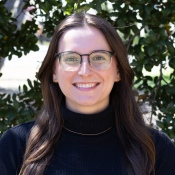
\includegraphics[height=0.9\textwidth]{static_figures/sequoia.jpg}\\
    Sequoia Andrade
\end{minipage}
\begin{minipage}[t]{0.24\textwidth}
    \centering
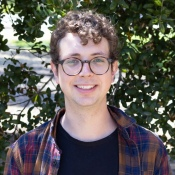
\includegraphics[height=0.9\textwidth]{static_figures/lucas.jpg}\\
Lucas Schwengber
\end{minipage}

}

\hrulefill

\textbf{Preprint and \texttt{R} package (hopefully) coming soon!}


\end{frame}

%%%%%%%%%%%%%%%%%%%%%%%%%%%%%%%%%%%%%%%%
%%%%%%%%%%%%%%%%%%%%%%%%%%%%%%%%%%%%%%%%
%%%%%%%%%%%%%%%%%%%%%%%%%%%%%%%%%%%%%%%%





%%%%%%%%%%%%%%%%%%%%%%%%%%%%%%%%%%%%%%%%%%%%%%%%%%%%%%%%%%%%%%%%%%%%%%%%%%%
%%%%%%%%%%%%%%%%%%%%%%%%%%%%%%%%%%%%%%%%%%%%%%%%%%%%%%%%%%%%%%%%%%%%%%%%%%%
%%%%%%%%%%%%%%%%%%%%%%%%%%%%%%%%%%%%%%%%%%%%%%%%%%%%%%%%%%%%%%%%%%%%%%%%%%%

\sectionslide{Extra slides}


\begin{frame}[allowframebreaks]{References}

\renewcommand*{\bibfont}{\normalfont\tiny}

%\footnotesize

% \bibliographystyle{plainnat}
% Hide the references header
% https://tex.stackexchange.com/questions/22645/hiding-the-title-of-the-bibliography/370784
% \begingroup
% \renewcommand{\section}[2]{}%
% \bibliography{references}
% \endgroup

\printbibliography[heading=none]

\end{frame}







%%%%%%%%%%%%%%%%%%%%%%%%%%%%%%%%%%%%%%%%%%%%%%%%%%%%%%%%%%%%%%%%%
%%%%%%%%%%%%%%%%%%%%%%%%%%%%%%%%%%%%%%%%%%%%%%%%%%%%%%%%%%%%%%%%%
%%%%%%%%%%%%%%%%%%%%%%%%%%%%%%%%%%%%%%%%%%%%%%%%%%%%%%%%%%%%%%%%%

\begin{frame}[t]{Frequentist variance estimation}


Let $\varemp{\cdot}$ denote the sample variance.

\begin{block}{Calibration weighting standard errors sketch:
    \footnote{E.g.~, \textcite{deville:1993:generalizedraking,fuller:2011:sampling}.}
}

If we have $\muhatcw = \surcol{\meansur \w_i \y_i}$ and a
consistent residual estimate $\surcol{\varepsilon_i}$, then

$$
\varemp{\surcol{\w_i \varepsilon_i}} \approx \var{}{\sqrt{\Nsur} \muhatcw}.
$$

\end{block}

\only<2->{

\begin{block}{MrPlew Standard error consistency theorem sketch (Our contribution):\footnote{
This is essentially a corollary of our earlier work on the Bayesian infinitesimal jackknife.\footcite{giordano:2024:bayesij}
}}

For Bayesian hierarchical logictic regression, define
$\surcol{\varepsilon_i = \y_i - \expect{\post}{\m(\x_i^\trans \theta)}}$.
% \quad\textrm{and}\quad
% \surcol{\psi_i := \Nsur \w_i^\mrp \varepsilon_i}.

We state mild conditions under which, as $\Nsur \rightarrow \infty$,
for some $\tarcol{\mu_\infty}$ and variance $V$,
$$
\begin{aligned}
    \sqrt{\Nsur}\left(\muhatmrp - \tarcol{\mu_\infty} \right) \rightarrow{}&
    \mathcal{N}\left(0, V\right)
    \quad\textrm{ and }\\
    \varemp{ \surcol{\w_i^\mrp \varepsilon_i}}
%\surcol{\meansur (\psi_i - \overline{\psi})^2}
    \rightarrow{} V.
\end{aligned}
$$
\end{block}

\textbf{The use of $\surcol{\w_i^\mrp}$ is analogous to the use of $\surcol{\w_i}$
for frequentist variance estimation.}
}

\end{frame}

%%%%%%%%%%%%%%%%%%%%%%%%%%%%%%%%%%%%%%%%%%%%%%%%%%%%%%%%%%%%%%%%%
%%%%%%%%%%%%%%%%%%%%%%%%%%%%%%%%%%%%%%%%%%%%%%%%%%%%%%%%%%%%%%%%%
%%%%%%%%%%%%%%%%%%%%%%%%%%%%%%%%%%%%%%%%%%%%%%%%%%%%%%%%%%%%%%%%%


\begin{frame}[t]{Standard error estimation experiment}

\wholeslidefig{\BootstrapPlot{}}

%\vspace{-3em}
% It's last minute so put in the manual estimate of the time
\pause
$$
\begin{aligned}
    \textrm{Running fifty MCMC parametric bootstraps:}\quad & \approx 79 \textrm{ hours} \\
    \textrm{Computing approximate weights:}\quad &\AlexMrPawTimeSecs \textrm{ seconds}\\
\end{aligned}
$$
\end{frame}




%%%%%%%%%%%%%%%%%%%%%%%%%%%%%%%%%%%%%%%%%%%%%%%%%%%%%%%%%%%%%%%%%
%%%%%%%%%%%%%%%%%%%%%%%%%%%%%%%%%%%%%%%%%%%%%%%%%%%%%%%%%%%%%%%%%
%%%%%%%%%%%%%%%%%%%%%%%%%%%%%%%%%%%%%%%%%%%%%%%%%%%%%%%%%%%%%%%%%

\begin{frame}{Real Data: Lax Philips}
Analysis of national support for gay marriage.\footnote{Based on \textcite{kastellec:2010:laxmrp},
see also \textcite{lax:2009:gay}.}

\begin{itemize}
    %
    \item \textbf{Target population:} US Census Public Use Microdata Sample 2000
    \item \textbf{Survey population:} Combined national-level polls from 2004
    \item \textbf{Respose:}  ``Do you favor allowing gay and lesbian couples to marry legally?''
    \item For regressors, use race, gender, age, education, state, region,
        and continuous statewide religion and political characteristics, including
        some analyst--selected interactions.
    %
\end{itemize}

$$
\begin{aligned}
    \textrm{Survey observations:} &&  \surcol{\Nsur} ={}& \LaxNSur  \\
    \textrm{Target observations (rows):} &&  \tarcol{\Ntar} ={}& \LaxNTar \\
    \\
    \textrm{Uncorrected survey mean:} && \surcol{\meansur \y_i} ={}& \LaxSurmean \\
    \textrm{Raking:} && \muhat_\cal ={}& \LaxRaking \\
    \textrm{MrP:} && \muhat_\mrp ={}& \LaxMrp
        \quad(\textrm{Post. sd} = \LaxMrpSD)\\
\end{aligned}
$$
%
\end{frame}



%%%%%%%%%%%%%%%%%%%%%%%%%%%%%%%%%%%%%%%%%%%%%%%%%%%%%%%%%%%%%%%%%
%%%%%%%%%%%%%%%%%%%%%%%%%%%%%%%%%%%%%%%%%%%%%%%%%%%%%%%%%%%%%%%%%
%%%%%%%%%%%%%%%%%%%%%%%%%%%%%%%%%%%%%%%%%%%%%%%%%%%%%%%%%%%%%%%%%



\begin{frame}{Covariate balance for primary effects}
\LaxImbalancePrimary{}
\end{frame}


\begin{frame}{Covariate balance for interaction effects}
\LaxImbalanceInteraction{}
\end{frame}




\begin{frame}[t]{Predictions}
    \LaxPredictionFigOne{}
\end{frame}


\begin{frame}[t]{Predictions and actual MCMC results}
    \LaxPredictionFigTwo{}
    \vspace{-3em}
    $$
    \begin{aligned}
        \textrm{Running ten MCMC refits:}\quad & \LaxRefitTimeHours \textrm{ hours} &
        \textrm{Computing approximate weights:}\quad &\LaxMrPawTimeSecs \textrm{ seconds}\\
    \end{aligned}
    $$
\end{frame}



%%%%%%%%%%%%%%%%%%%%%%%%%%%%%%%%%%%%%%%%%%%%%%%%%%%%%%%%%%%%%%%%%
%%%%%%%%%%%%%%%%%%%%%%%%%%%%%%%%%%%%%%%%%%%%%%%%%%%%%%%%%%%%%%%%%
%%%%%%%%%%%%%%%%%%%%%%%%%%%%%%%%%%%%%%%%%%%%%%%%%%%%%%%%%%%%%%%%%




\def\res{\varepsilon}
\def\w{w}
\def\wtil{\tilde{\w}}
\def\reshat{\hat{\res}}

\def\methodrow#1#2#3{
\begin{minipage}[t]{0.15\textwidth}
    \centering
    %\rotatebox{90}{#1}
    #1
\end{minipage}
\hfill
\begin{minipage}[t]{0.4\textwidth}
    \centering
    \vspace{-2em}
    #2
    \pause
\end{minipage}
\hfill
\begin{minipage}[t]{0.4\textwidth}
    \centering
    \vspace{-2em}
    #3
    \pause
\end{minipage}
}


\def\methodspacer{
    \vspace{1em}
    \hrule
    \vspace{1em}
}

\begin{frame}{Some generalized diagnostics}

\vspace{2em}
\methodrow{\,}{\textbf{Regression}}{\textbf{General models}}

\methodrow{Consistency /\\ Unbiased}
{
$$
\begin{aligned}
    \y ={}& \theta^\trans \x + \res \\
    \ytil ={}& (\theta + \delta)^\trans \x + \res \\
    \thetahat(\ytil) \eqcheck{}& \thetahat(\y) + \delta
\end{aligned}
$$
}{
$$
\begin{aligned}
    \y ={}& \f(\x, \varepsilon, \theta) \\
    \ytil ={}& \f(\x, \varepsilon, \theta + \delta) \\
    \thetahat(\ytil) \eqcheck{}& \thetahat(\y) + \delta
\end{aligned}
$$
}

\methodspacer

\methodrow{Exogonous\\residuals}
{
$$
\begin{aligned}
    \y ={}& \theta^\trans \x + \res \\
    \ytil ={}& \y + \res \z \\
    \thetahat(\ytil) \eqcheck{}& \thetahat(\y)
\end{aligned}
$$
}{
$$
\begin{aligned}
    \y \sim{}& \p(\y \vert \x) \textrm{ and } \p(\x) ={} \w \\
    \wtil ={}& \w + \delta z \\
    \thetahat(\wtil) \eqcheck{}& \thetahat(\w)
\end{aligned}
$$
}


\methodspacer


\methodrow{Fisher information}
{
$$
\begin{aligned}
    %\y ={}& \theta^\trans \x + \res \\
    \mathcal{I} :={}& \textrm{Fisher information}\\
    \Sigma :={}& \textrm{Score covariance} \\
    \mathcal{I}^{-1} \eqcheck{}& \Sigma
\end{aligned}
$$
}{
$$
\begin{aligned}
    \y \sim{}& \p(\y \vert \theta) \\
    \ytil \sim{}& \textrm{Importance sample }\y\\
    &\textrm{ using }\wtil ={} \frac{\p(\y \vert \thetahat + \delta)}{\p(\y \vert \thetahat)} \\
    \thetahat(\wtil) \eqcheck{}& \thetahat(1) + \delta
\end{aligned}
$$
}


\vspace{2em}


\end{frame}



%%%%%%%%%%%%%%%%%%%%%%%%%%%%%%%%%%%%%%%%
%%%%%%%%%%%%%%%%%%%%%%%%%%%%%%%%%%%%%%%%
%%%%%%%%%%%%%%%%%%%%%%%%%%%%%%%%%%%%%%%%

\begin{frame}{Weights by education for the Name Change analysis}

    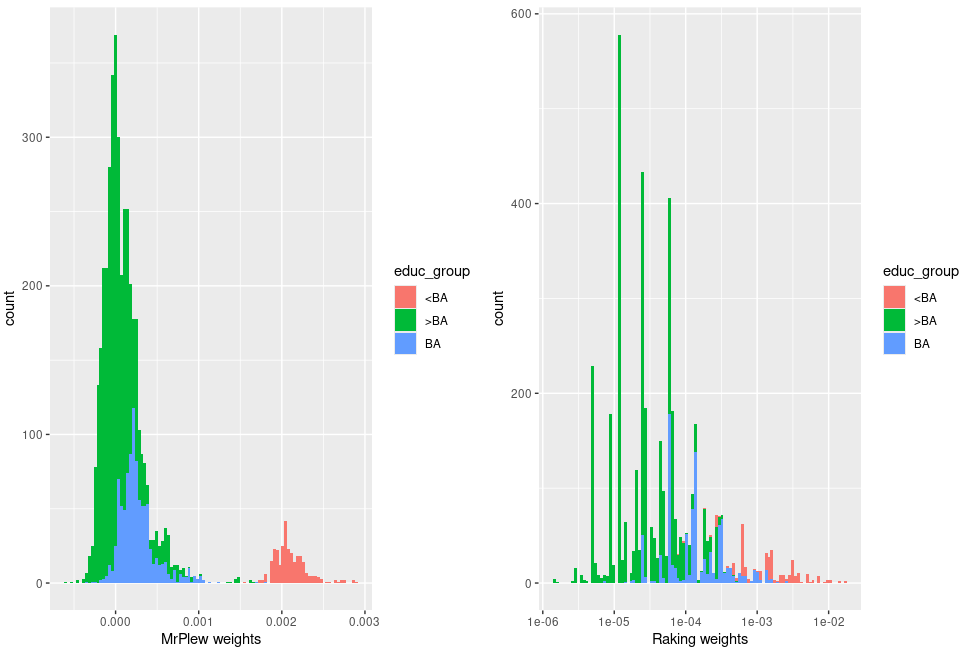
\includegraphics[width=0.8\textwidth]{static_figures/w_educ_hist.png}
\end{frame}



%%%%%%%%%%%%%%%%%%%%%%%%%%%%%%%%%%%%%%%%
%%%%%%%%%%%%%%%%%%%%%%%%%%%%%%%%%%%%%%%%
%%%%%%%%%%%%%%%%%%%%%%%%%%%%%%%%%%%%%%%%










\end{document}
